\documentclass[11pt,a4paper]{article}

% Packages
\usepackage[utf8]{inputenc}
\usepackage[spanish, es-tabla]{babel}
\usepackage{parskip}
\usepackage{enumerate}
\usepackage{graphicx}
\usepackage{subfigure}
\usepackage{float}
\usepackage{amsmath}
\usepackage{amssymb}
\usepackage{upgreek}
\usepackage{enumitem}
\usepackage{dsfont}
\usepackage{xfrac}
\usepackage{lmodern}
\usepackage{listings}

\usepackage[bookmarks=true,
					 bookmarksnumbered=false,
					 bookmarksopen=false,
					 colorlinks=true,
					 allcolors=blue,
					 urlcolor=blue]{hyperref}

\usepackage[ruled]{algorithm2e}
\SetKwInOut{Parameter}{parameter}

\usepackage{array}
\newcolumntype{N}{>{\centering\arraybackslash}m{0.5cm}}
\newcolumntype{M}{>{\centering\arraybackslash}m{1cm}}

\usepackage[left=2cm, right=2cm, top=2cm, bottom=2cm]{geometry}

\begin{document}\pagenumbering{arabic}
\begin{titlepage}
\centering
\includegraphics[width=0.15\textwidth]{/Users/pedrors/Desktop/DGIIM/Latex/UGR}\par\vspace{1cm}
{\scshape\LARGE Universidad de Granada \par}
\vspace{1cm}
\vspace{1.5cm}
{\huge\bfseries Estadística Multivariante\par}
\vspace{1cm}
{\large\bfseries Práctica Final\par}
\vspace{2cm}
{\Large\itshape Pedro Ramos Suárez\par}
\vfill
Doble Grado de Ingeniería Informática y Matemáticas
\vfill
{\large \today\par}
\end{titlepage}

\tableofcontents
\newpage
\section{Resumen}
En esta práctica realizo un análisis exploratorio de un conjunto de datos formado por 8 indicadores económicos de 13 empresas, estudiando la información para realizar:
\begin{itemize}
	\item Análisis exploratorio univariante: Se elabora un análisis descriptivo clásico y un análisis de supuesto de normalidad.
	\item Análisis exploratorio multivariante: Se estudia la correlación entre variables, reducción de la dimensión mendiante variables observables y latentes (ACP y AF), así como la normalidad multivariante de los datos.
\end{itemize}

Finalmente, se realiza un clustering con el algoritmo de K-Medias.

\section{Introducción}
Realizo el análisis exploratorio en \emph{DB\_2}, una base de datos propuesta, que contiene datos de 13 empresas que se ha clasificado según las puntuaciones obtenidas en 8 indicadores económicos.

Primero, he realizado todo el tratamiento de datos. Para ello, he eliminado los valores perdidos, que pertenecían a una instancia errónea, ya que teníamos 14 en lugar de las 13 indicadas en la descripción de la base de datos, y esta instancia, además de los valores perdidos, tenía valores muy lejanos al resto de instancias, lo cuál me ha hecho suponer que es errónea. Luego he realizado el tratamiento de outliers, he realizado un análisis descriptivo clásico (obteniendo las medias, cuartiles, coeficiente de simetría, etc), y finalmente he estudiado la normalidad de los datos.

Luego, he realizado un análisis exploratorio multivariante, comenzando por comprobar la correlación entre las variables, seguido del estudio de la dimensión mediante variables observables, obteniendo un total de 3 componentes, y mediante variables latentes, en el cuál también he obtenido un total de 3 factores. Además, estudio la normalidad de los datos.

Finalmente, se realiza un análisis cluster agrupando los datos formando clusters según la homogeneidad a través de K-Medias. Los resultados que obtenemos en esta última fase no son muy concluyentes, seguramente debido al pequeño número de datos.

\section{Materiales y métodos}
\subsection{Materiales}
La base de datos elegida contiene un grupo constituido por 13 empresas que se ha clasificado según las puntuaciones obtenidas en 8 indicadores económicos.
\begin{itemize}
\item X1: Indicador de volumen de facturación de la empresa.
\item X2: Indicador del nivel de nueva contratación.
\item X3: Indicador del total de clientes
\item X4: Indicador de beneficios de la empresa.
\item X5: Indicador de nivel de retribución salarial de los empleados.
\item X6: Indicador de nivel de organización empresarial dentro de la empresa.
\item X7: Indicador de nivel de relaciones con otras empresas.
\item X8: Indicador de nivel de equipamiento (ordenadores, maquinaria, etc.).
\end{itemize}

La información esta base de datos queda resumida en:
\begin{verbatim}
##        x1                  x2                x3               x4         
##  Min.   :    0.128   Min.   : 0.9444   Min.   : 2.167   Min.   : 0.0299  
##  1st Qu.:    3.360   1st Qu.: 9.3298   1st Qu.: 9.208   1st Qu.: 4.2718  
##  Median :    7.799   Median :16.4244   Median :15.583   Median : 5.5994  
##  Mean   : 1436.674   Mean   :15.1342   Mean   :15.226   Mean   : 5.5835  
##  3rd Qu.:   11.321   3rd Qu.:21.1861   3rd Qu.:21.125   3rd Qu.: 7.1857  
##  Max.   :20023.000   Max.   :25.4261   Max.   :28.167   Max.   :11.3959  
##                                                                          
##        x5               x6               x7               x8        
##  Min.   : 2.557   Min.   : 6.135   Min.   : 1.064   Min.   : 3.949  
##  1st Qu.: 3.678   1st Qu.:10.042   1st Qu.: 3.982   1st Qu.: 6.833  
##  Median : 5.408   Median :11.235   Median : 5.584   Median : 8.103  
##  Mean   : 5.314   Mean   :20.220   Mean   : 6.598   Mean   :13.074  
##  3rd Qu.: 5.908   3rd Qu.:31.449   3rd Qu.:10.160   3rd Qu.:20.154  
##  Max.   :10.037   Max.   :43.278   Max.   :12.374   Max.   :26.571  
##                                    NA's   :1        NA's   :1
\end{verbatim}

Y tras eliminar los datos erróneos:
\begin{verbatim}
##        x1               x2                x3               x4         
##  Min.   : 0.128   Min.   : 0.9444   Min.   : 2.167   Min.   : 0.0299  
##  1st Qu.: 2.476   1st Qu.: 8.6931   1st Qu.: 8.667   1st Qu.: 4.0673  
##  Median : 7.584   Median :14.8487   Median :15.167   Median : 5.4044  
##  Mean   : 6.957   Mean   :14.9138   Mean   :15.167   Mean   : 5.3976  
##  3rd Qu.:10.734   3rd Qu.:21.7262   3rd Qu.:21.667   3rd Qu.: 6.5147  
##  Max.   :14.364   Max.   :25.4261   Max.   :28.167   Max.   :11.3959  
##        x5               x6               x7               x8        
##  Min.   : 2.557   Min.   : 6.135   Min.   : 1.064   Min.   : 3.949  
##  1st Qu.: 3.525   1st Qu.:10.170   1st Qu.: 3.982   1st Qu.: 6.833  
##  Median : 5.336   Median :11.374   Median : 5.584   Median : 8.103  
##  Mean   : 5.107   Mean   :21.006   Mean   : 6.598   Mean   :13.074  
##  3rd Qu.: 5.874   3rd Qu.:31.586   3rd Qu.:10.160   3rd Qu.:20.154  
##  Max.   :10.037   Max.   :43.278   Max.   :12.374   Max.   :26.571
\end{verbatim}

Podemos visualizarlos en el siguiente diagrama:
\begin{figure}[H]
\centering
\subfigure{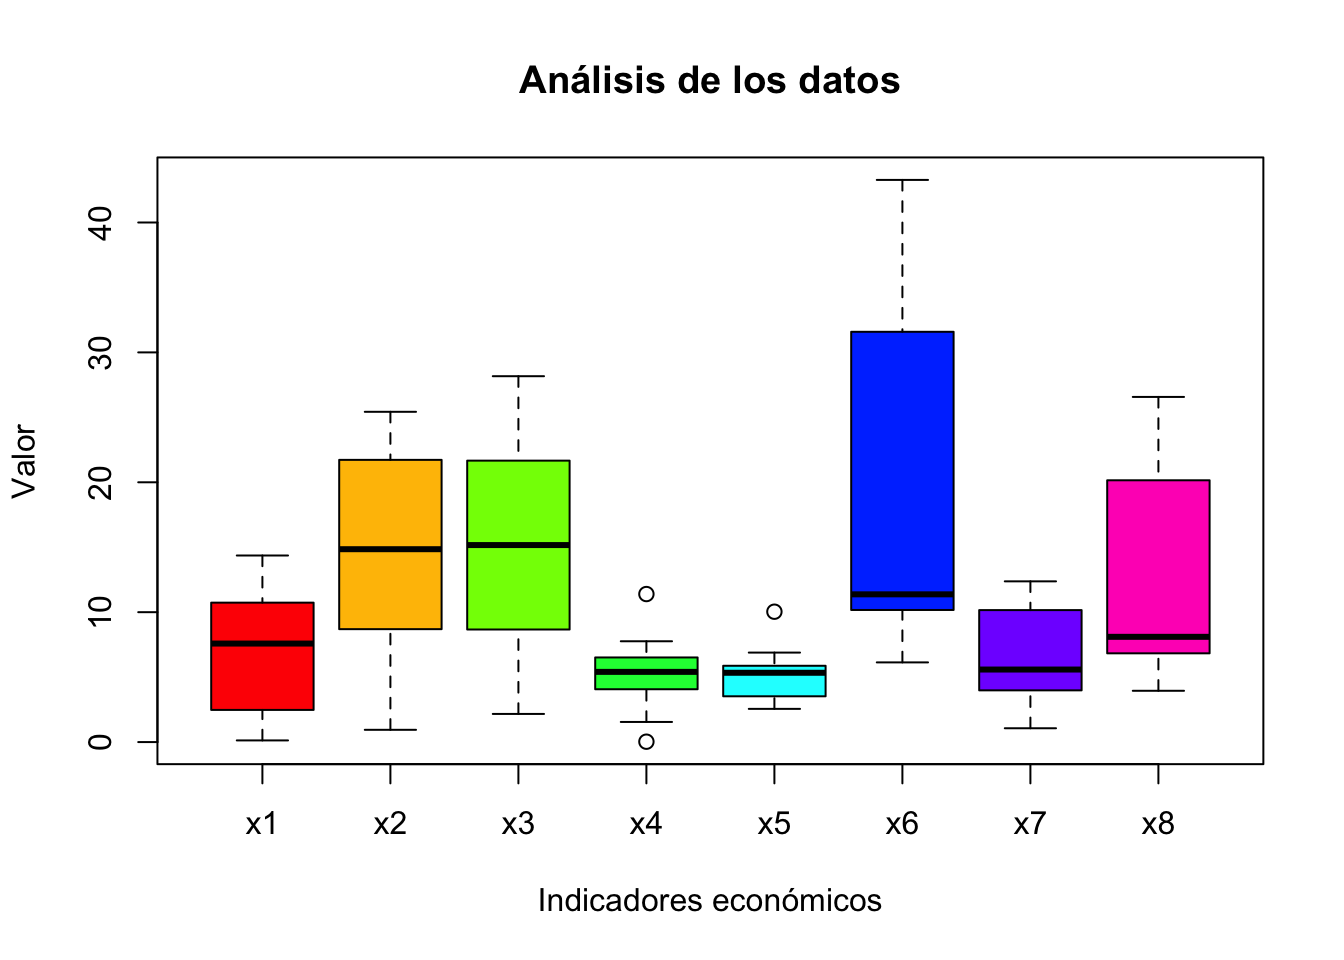
\includegraphics[width=0.4\textwidth]{../img/img1.png}}
\subfigure{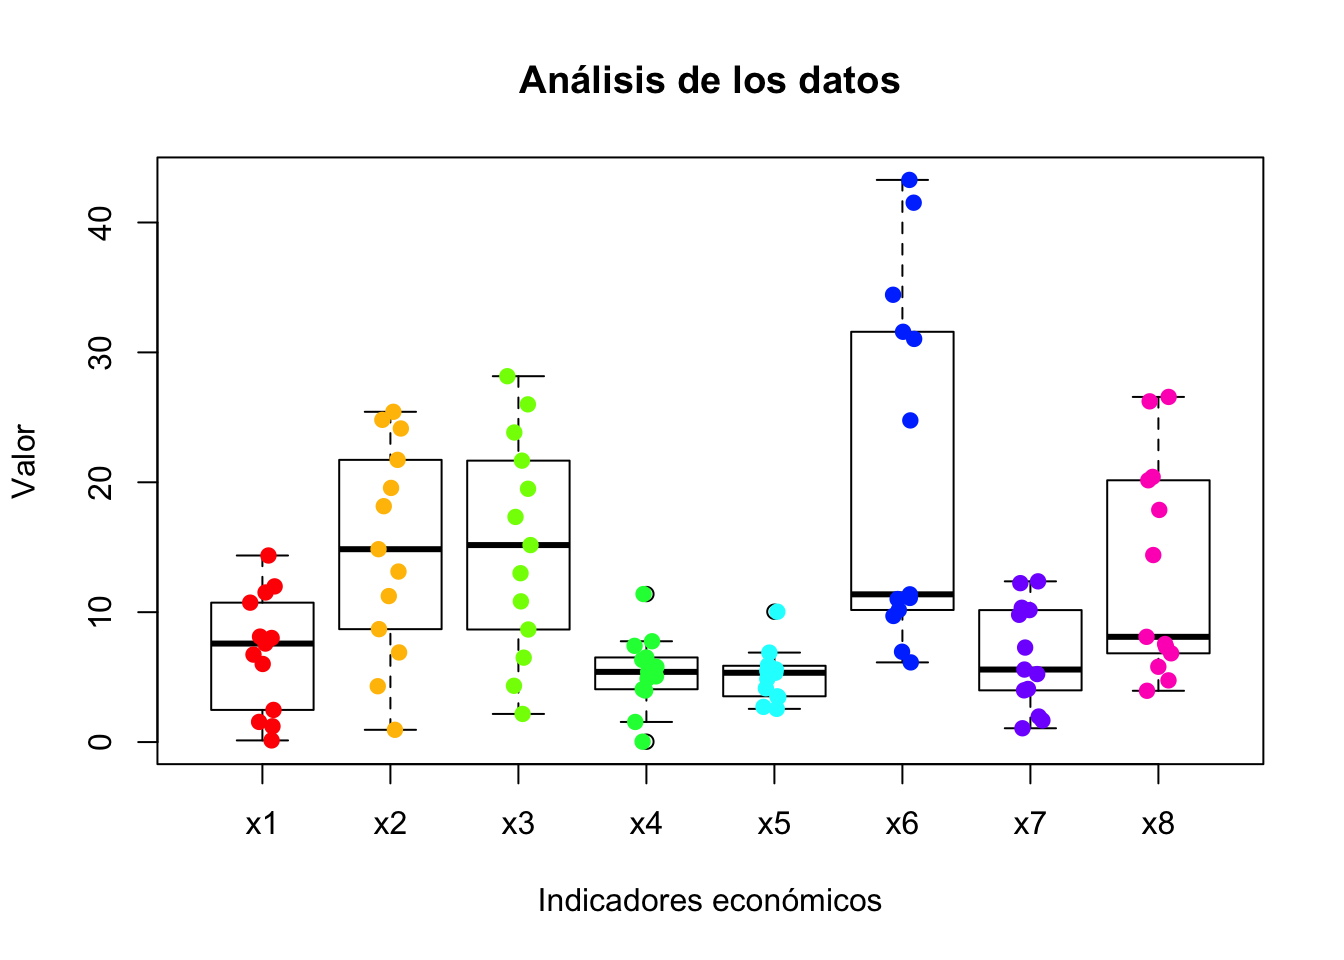
\includegraphics[width=0.4\textwidth]{../img/img2.png}}
\end{figure}

\subsection{Métodos estadísticos}
Pasamos ha discutir las distintas técnicas estadísticas utilizadas.

Para el análisis exploratorio univariante, hemos cargado y visualizado la estructura de los datos, a partir de los cuales hemos podido eliminar los valores perdidos. También hemos realizado un análisis descriptivo numérico clásico usando las funciones \emph{summary}, \emph{boxplot}, \emph{stripchart} y \emph{skewness}, con las cuales hemos obtenido las medidas de tendencia central, la dispersión, los cuartiles, la simetría, los diagramas de caja, ... Para el tratamiento de outliers, hemos utilizado \emph{check\_outliers}, además de comentar el método visto en clase. Finalmente, para el supuesto de normalidad, hemos utilizado \emph{colMeans} y \emph{scale}, y lo hemos visualizado con \emph{qqplot}.

Para el análisis exploratorio multivariante, se ha utilizado el test de Bartlett con \emph{cortest.bartlett} para estudiar la correlación entre las variables. Para el Análisis de Componentes Principales (ACP) se utiliza \emph{prcomp} y se visualiza con \emph{ggplot} y \emph{fviz\_pca}. Para el Análisis Funcional (AF), se utiliza otras funciones como \emph{fa} y \emph{factanal}, y para la visualización \emph{ggcorrplot}, \emph{scree}, \emph{parallel} y \emph{diagram}. Finalmente, para el análisis de normalidad se utilizan funciones de \emph{MVM} para realizar el test de Royston y el test de Henze-Zirkler.

Por último, para el clustering, se utiliza \emph{kmeans}.

\section{Resultados}
\subsection{Análisis exploratorio univariante}
Para estudiar el conjunto de datos calculamos el coeficiente de simetría:
\begin{lstlisting}[language=R]
skewness(datos)
\end{lstlisting}
\begin{verbatim}
##            x1            x2            x3            x4            x5 
## -6.571128e-02 -2.178143e-01  2.441493e-16  8.611432e-02  9.539367e-01 
##            x6            x7            x8 
##  4.214678e-01  1.014152e-01  4.874442e-01
\end{verbatim}

Para el estudio de outliers, podemos utilizar los plotboxes mostrados previamente o, en este caso, la función:
\begin{lstlisting}[language=R]
check_outliers(datos, method="mahalanobis")
\end{lstlisting}
\begin{verbatim}
## OK: No outliers detected.
## - Based on the following method and threshold: mahalanobis (26.12).
## - For variables: x1, x2, x3, x4, x5, x6, x7, x8
\end{verbatim}

Para estudiar el supuesto de normalidad estudiamos la distribución de las variables, obteniendo:
\begin{figure}[H]
\centering
\subfigure{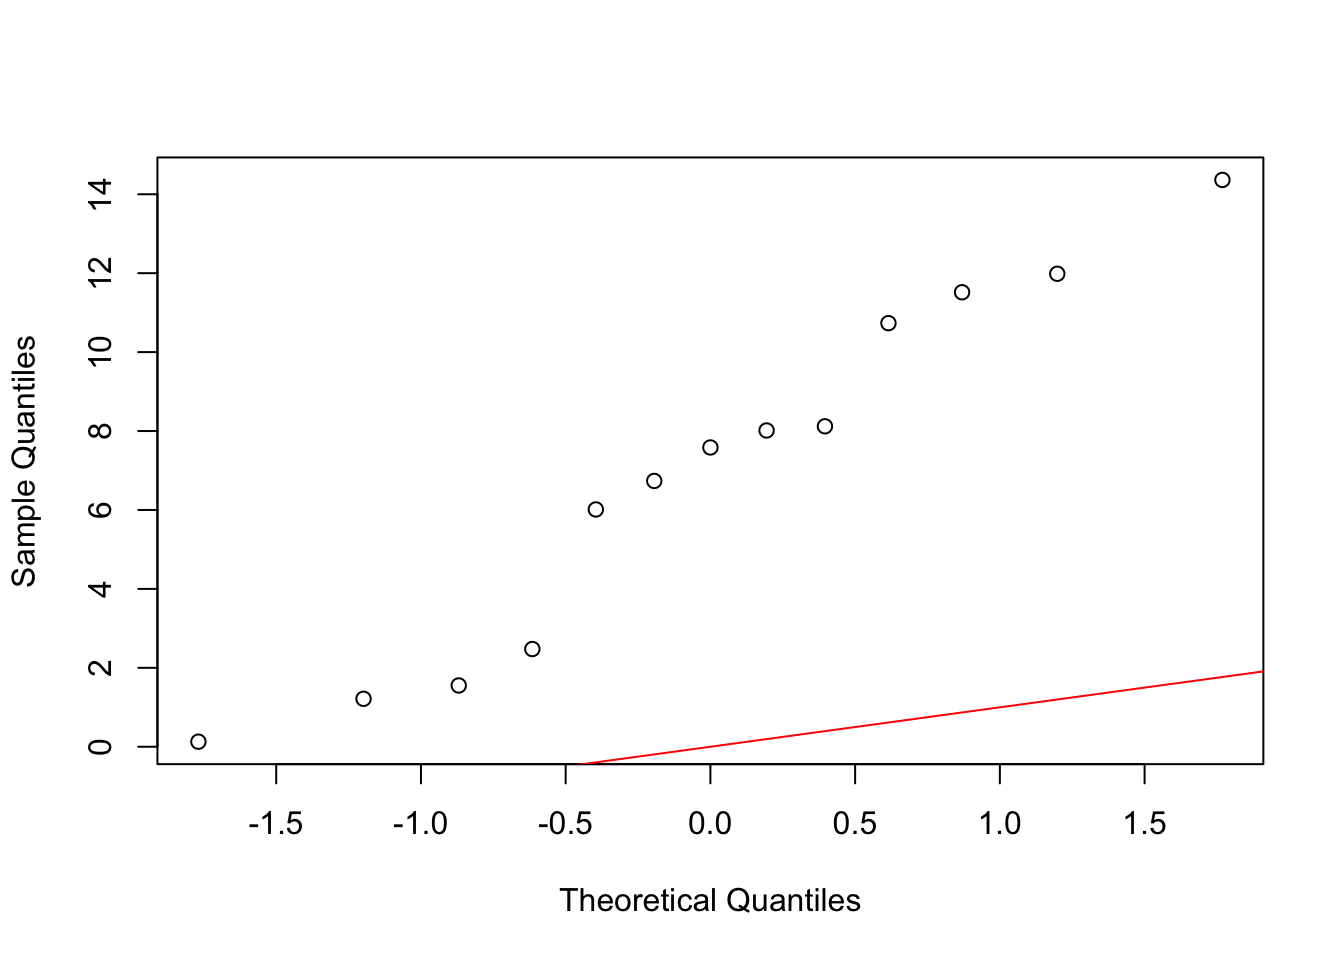
\includegraphics[width=0.2\textwidth]{../img/img3.png}}
\subfigure{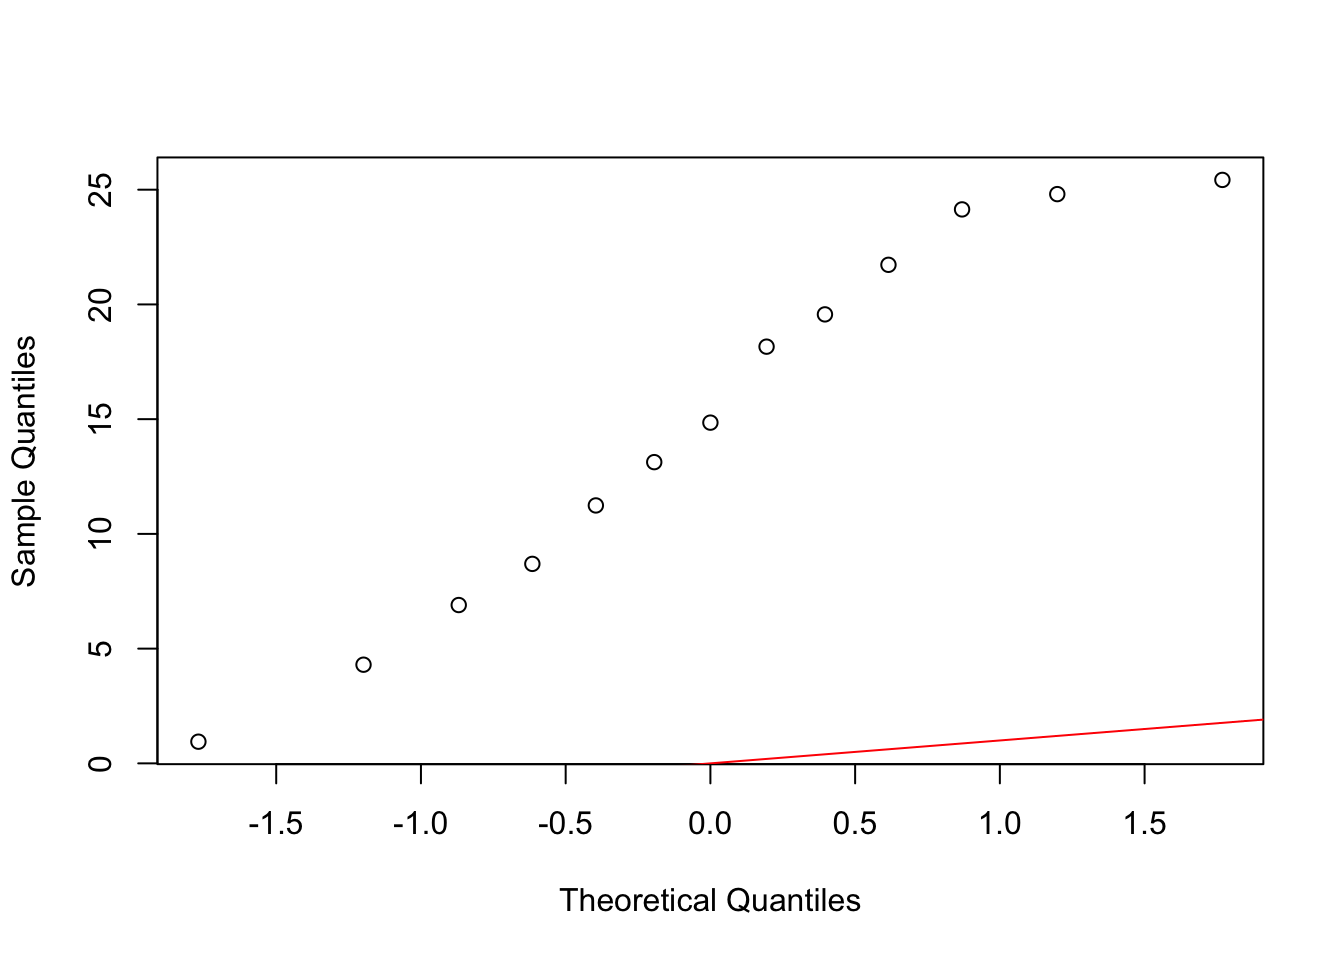
\includegraphics[width=0.2\textwidth]{../img/img4.png}}
\subfigure{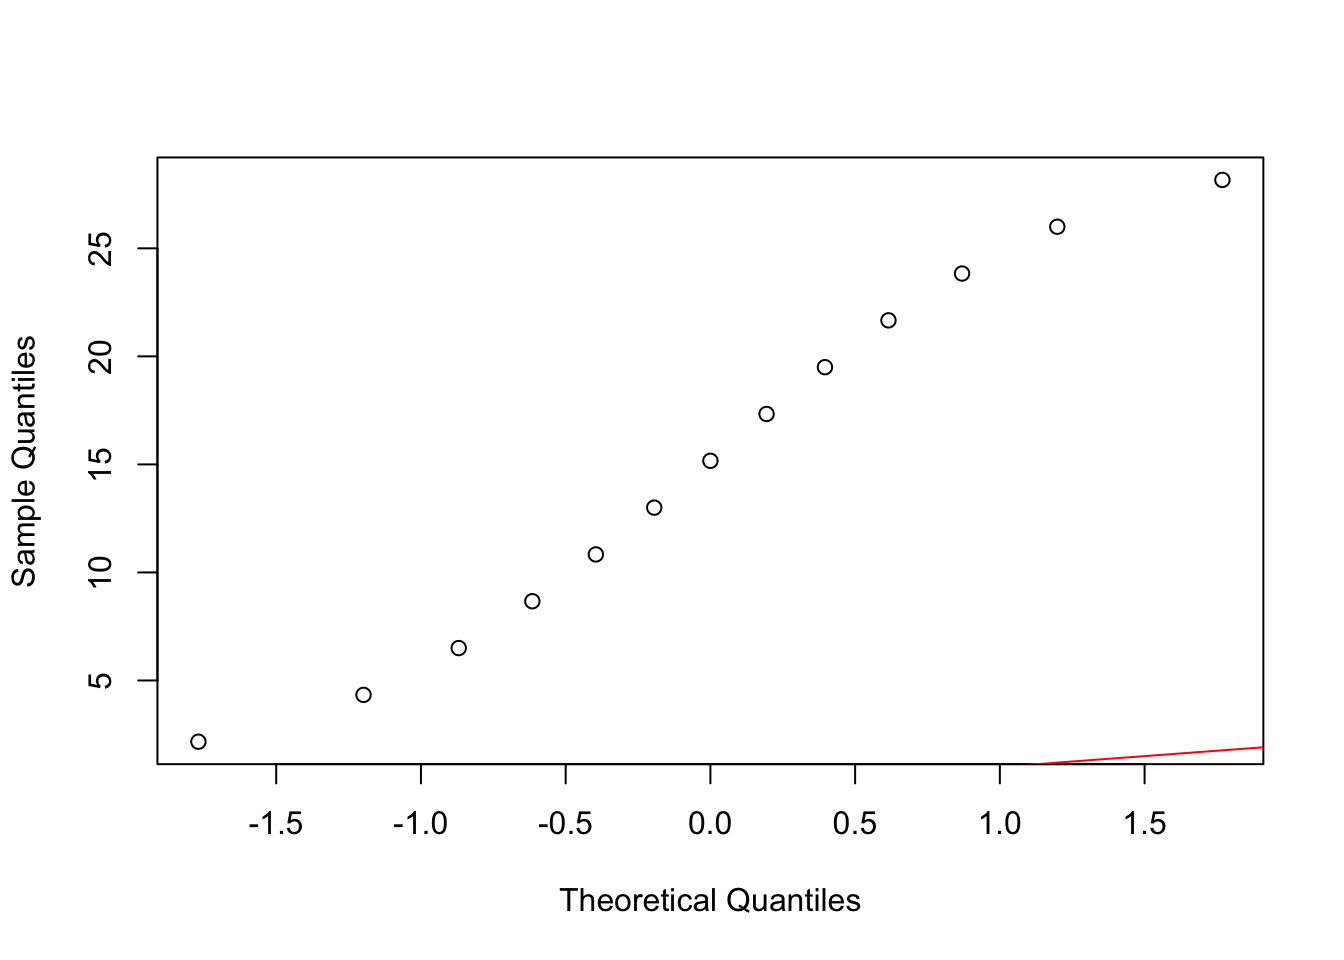
\includegraphics[width=0.2\textwidth]{../img/img5.png}}
\subfigure{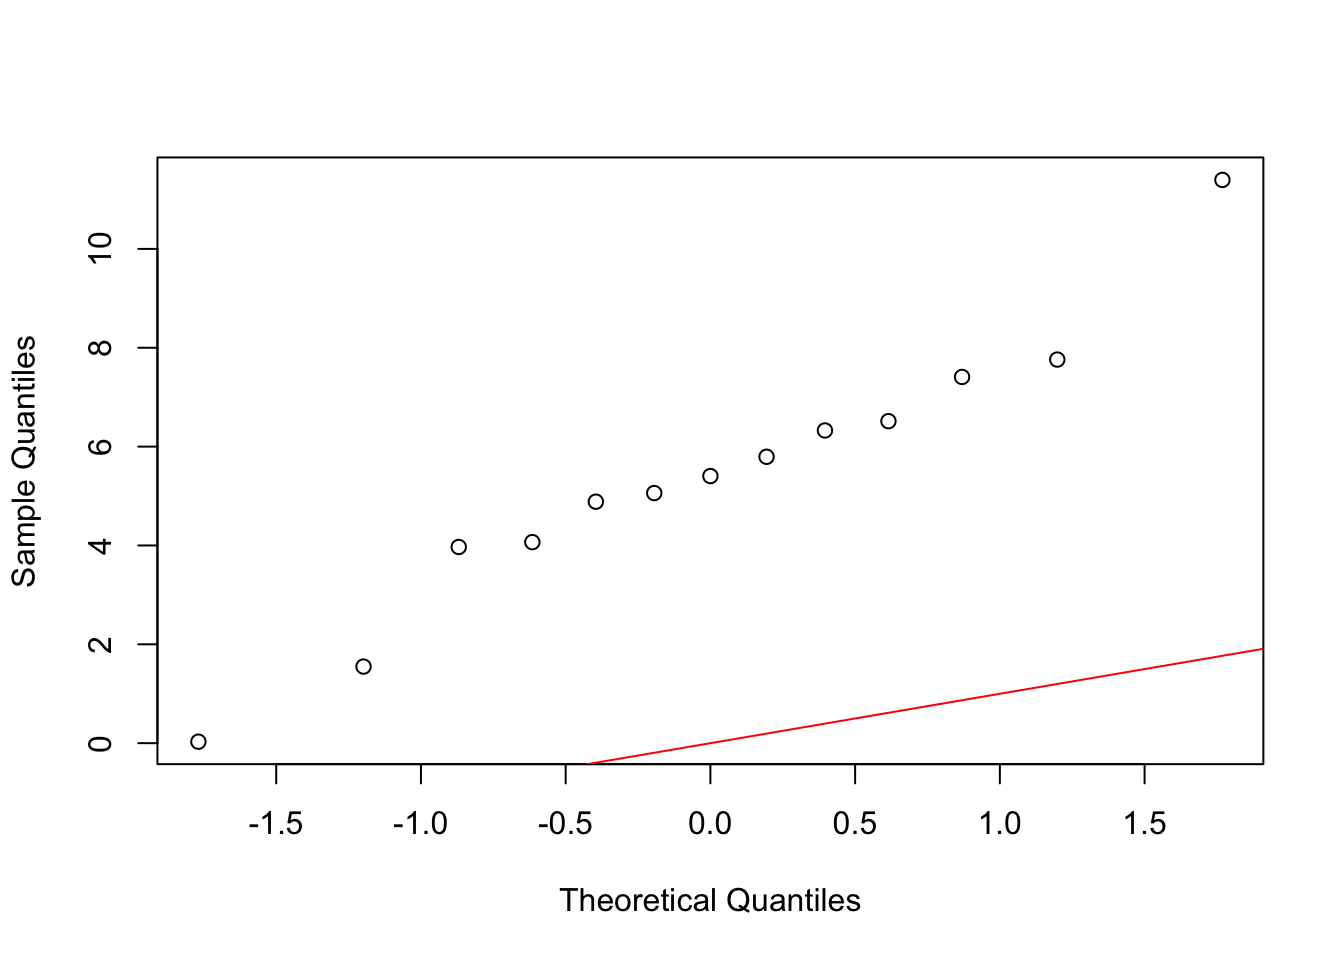
\includegraphics[width=0.2\textwidth]{../img/img6.png}}
\subfigure{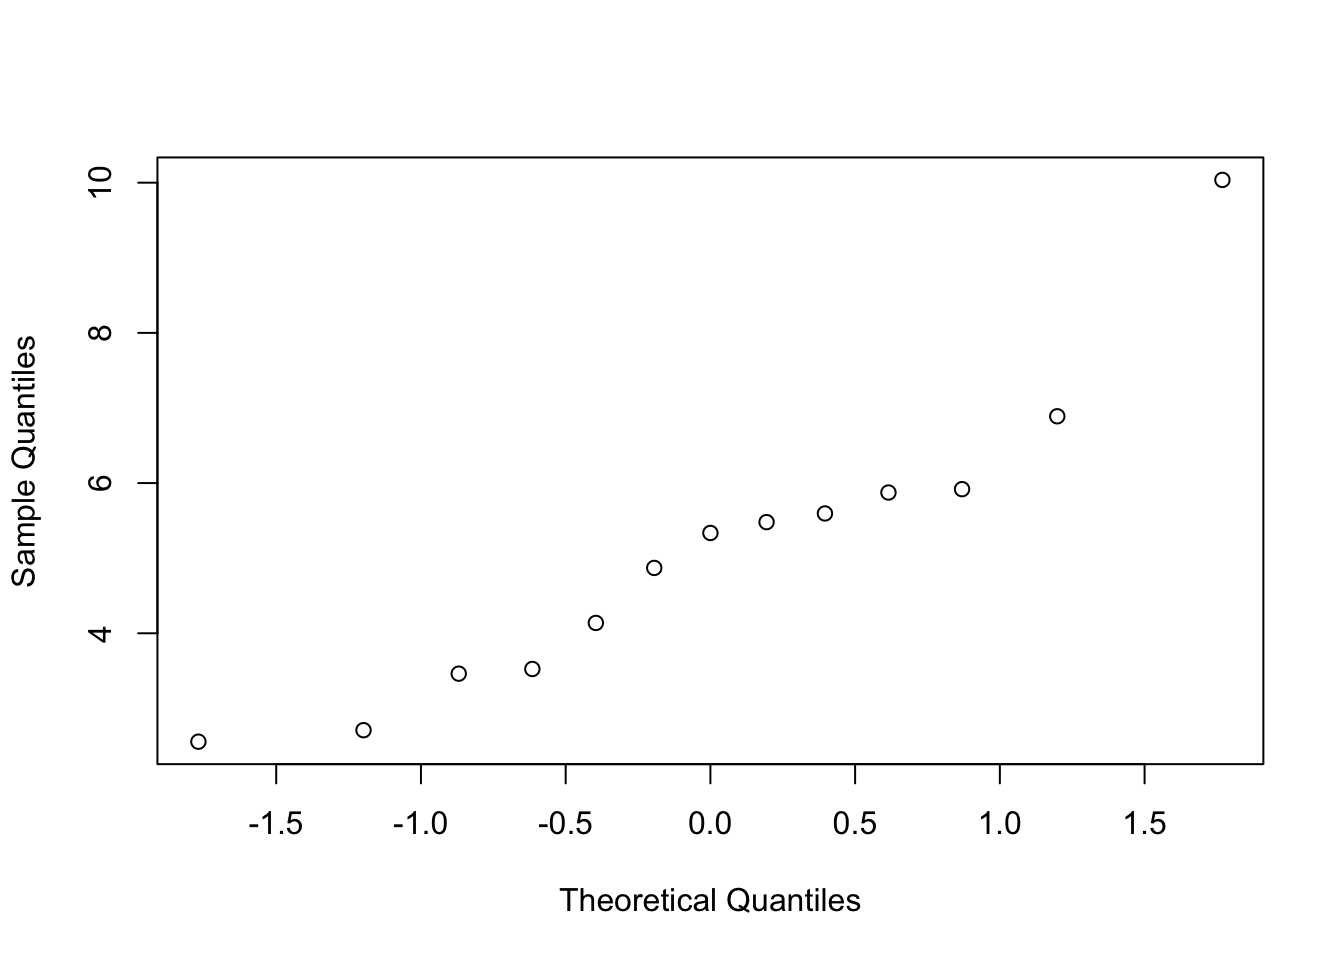
\includegraphics[width=0.2\textwidth]{../img/img7.png}}
\subfigure{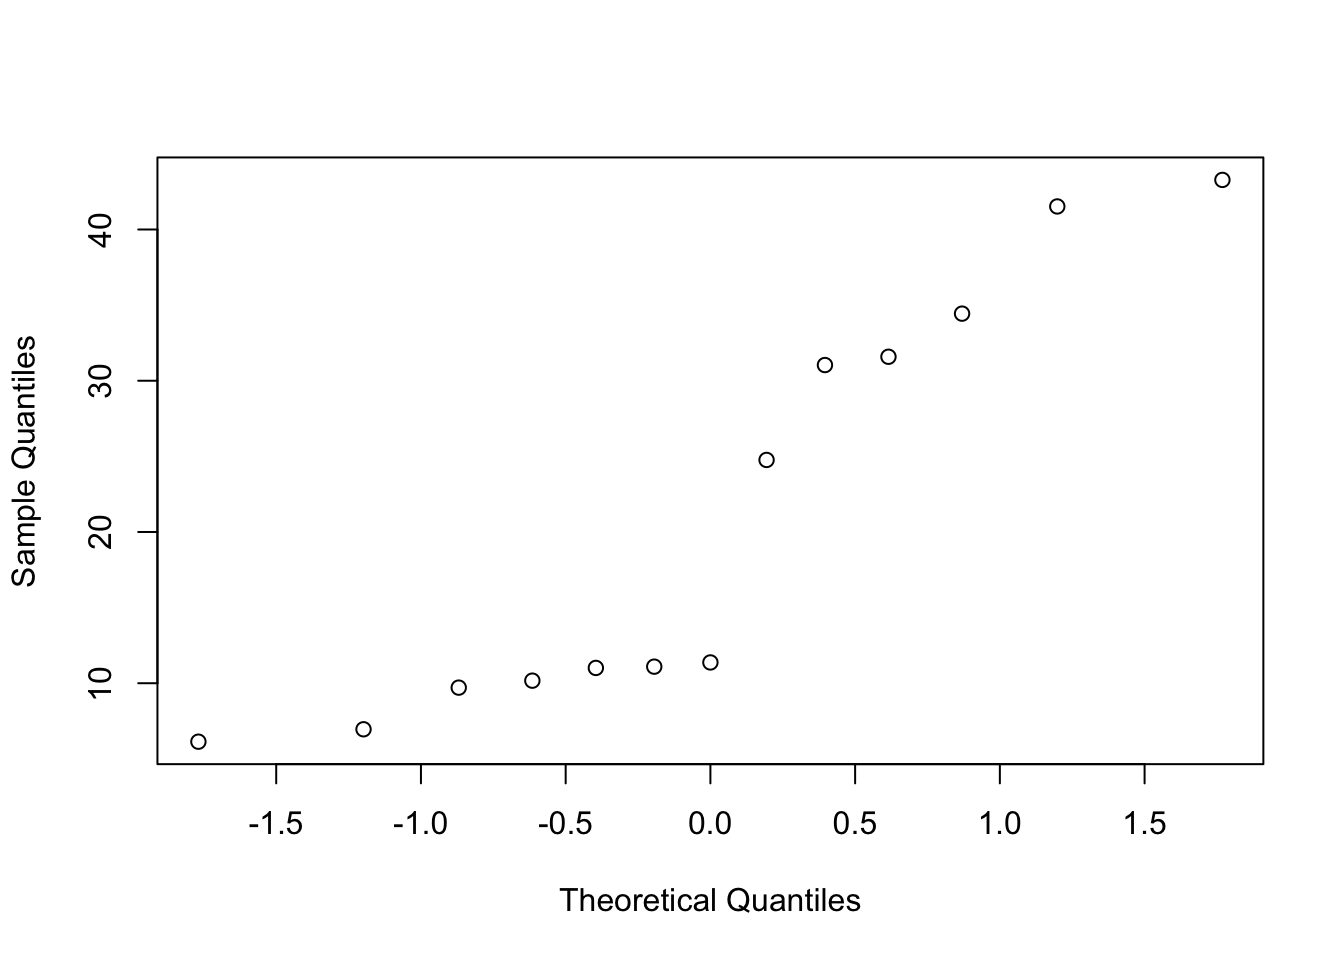
\includegraphics[width=0.2\textwidth]{../img/img8.png}}
\subfigure{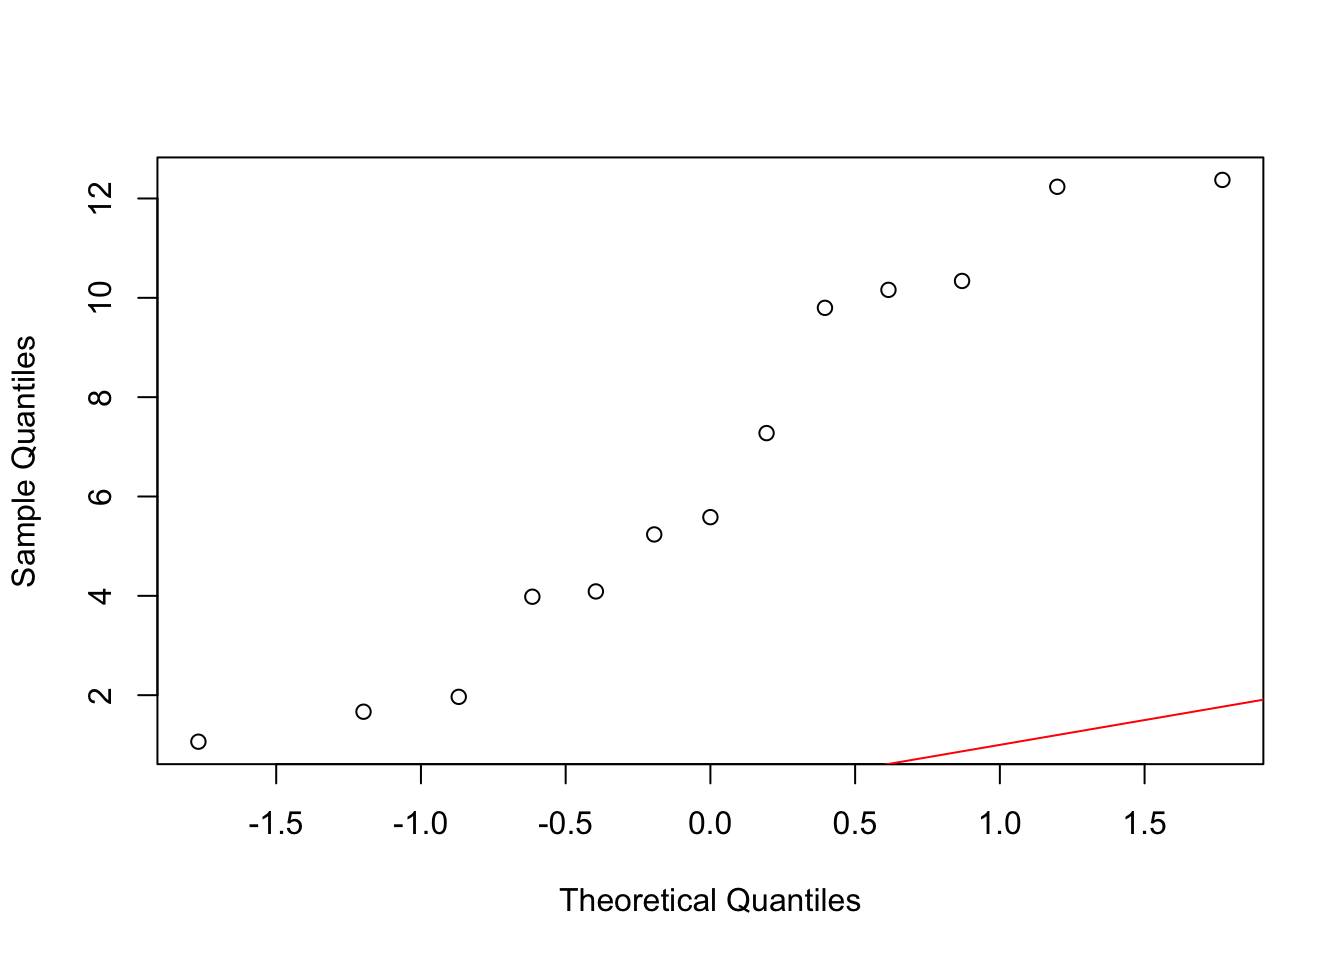
\includegraphics[width=0.2\textwidth]{../img/img9.png}}
\subfigure{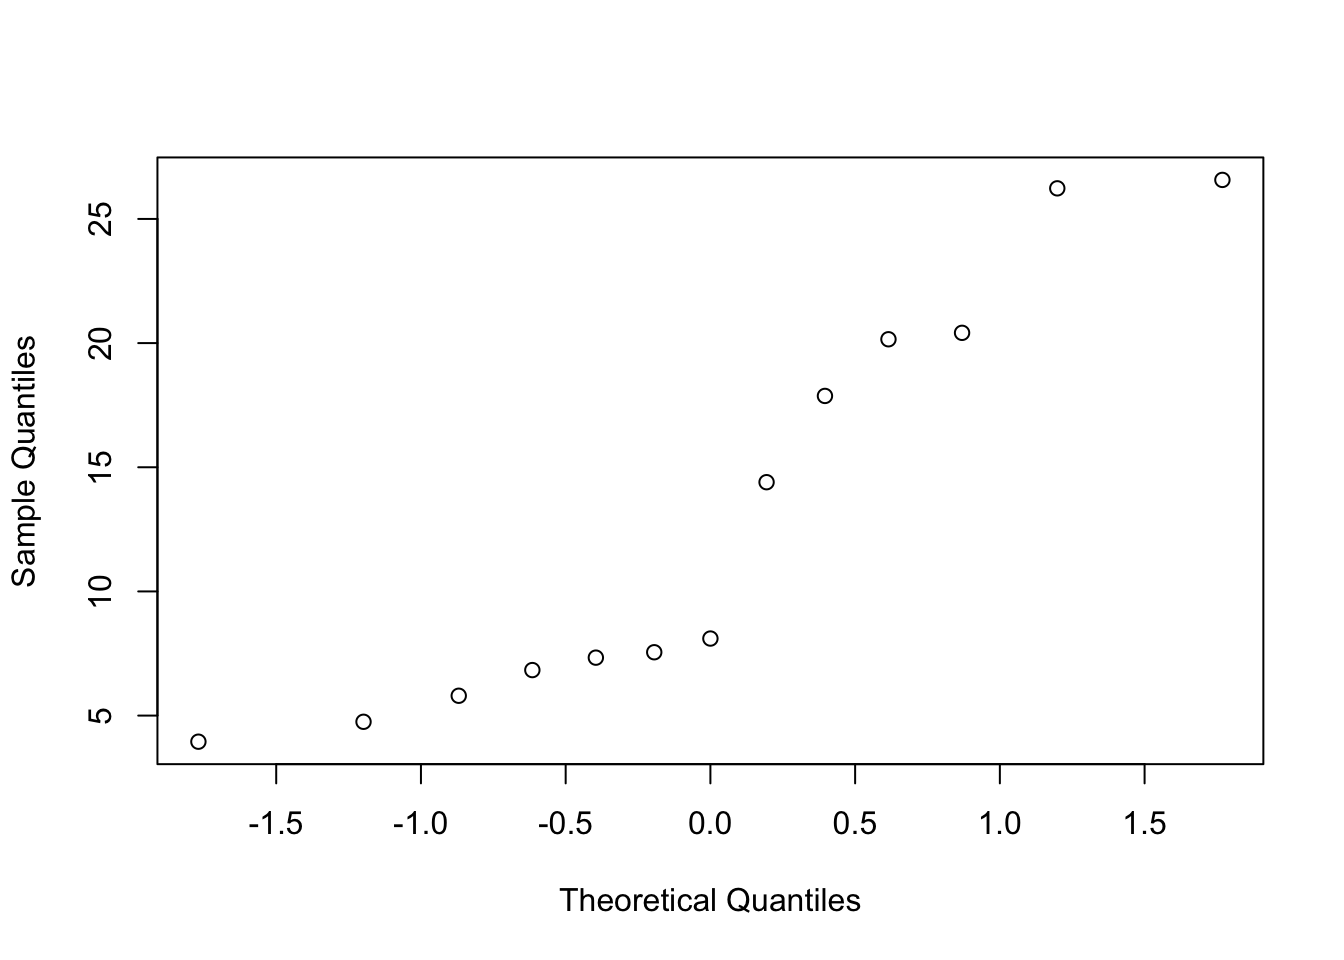
\includegraphics[width=0.2\textwidth]{../img/img10.png}}
\caption{Datos antes de normalizar}
\end{figure}

Como podemos ver que no están normalizados, utilizamos \emph{scale} para normalizarlos de donde obtenemos:
\begin{figure}[H]
\centering
\subfigure{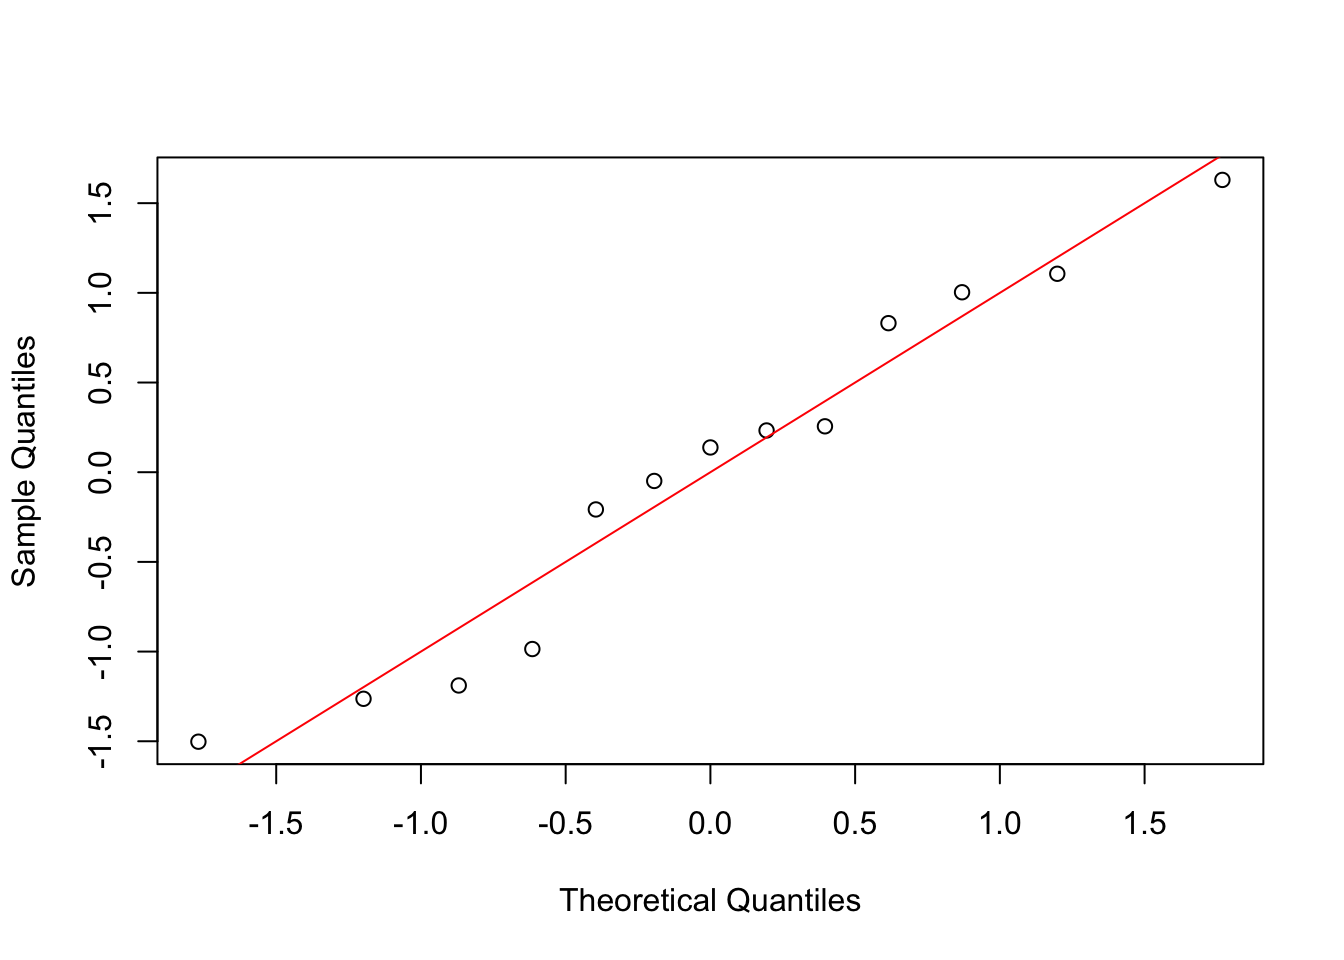
\includegraphics[width=0.2\textwidth]{../img/img11.png}}
\subfigure{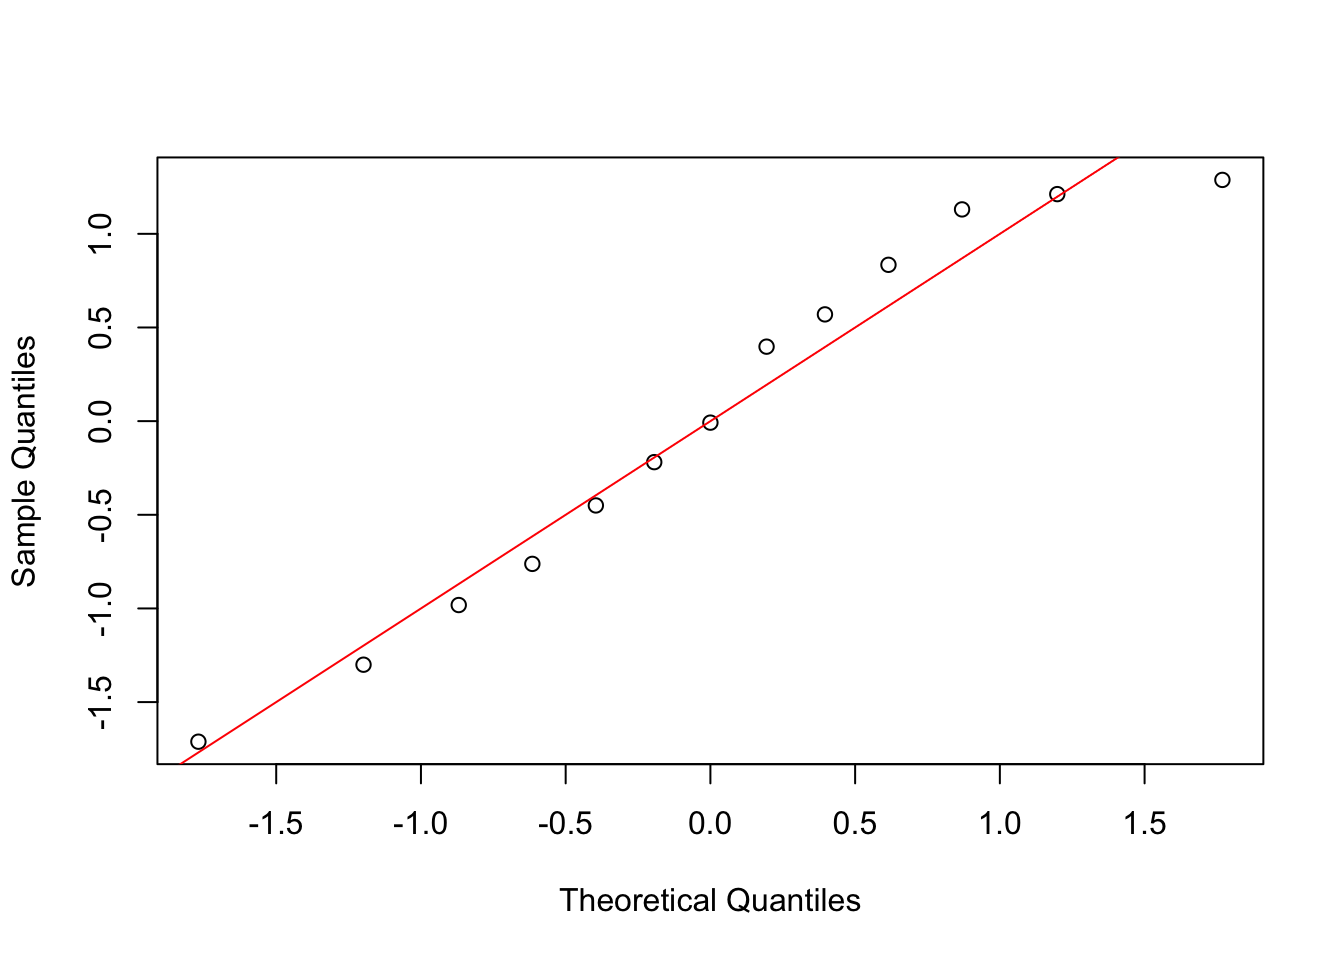
\includegraphics[width=0.2\textwidth]{../img/img12.png}}
\subfigure{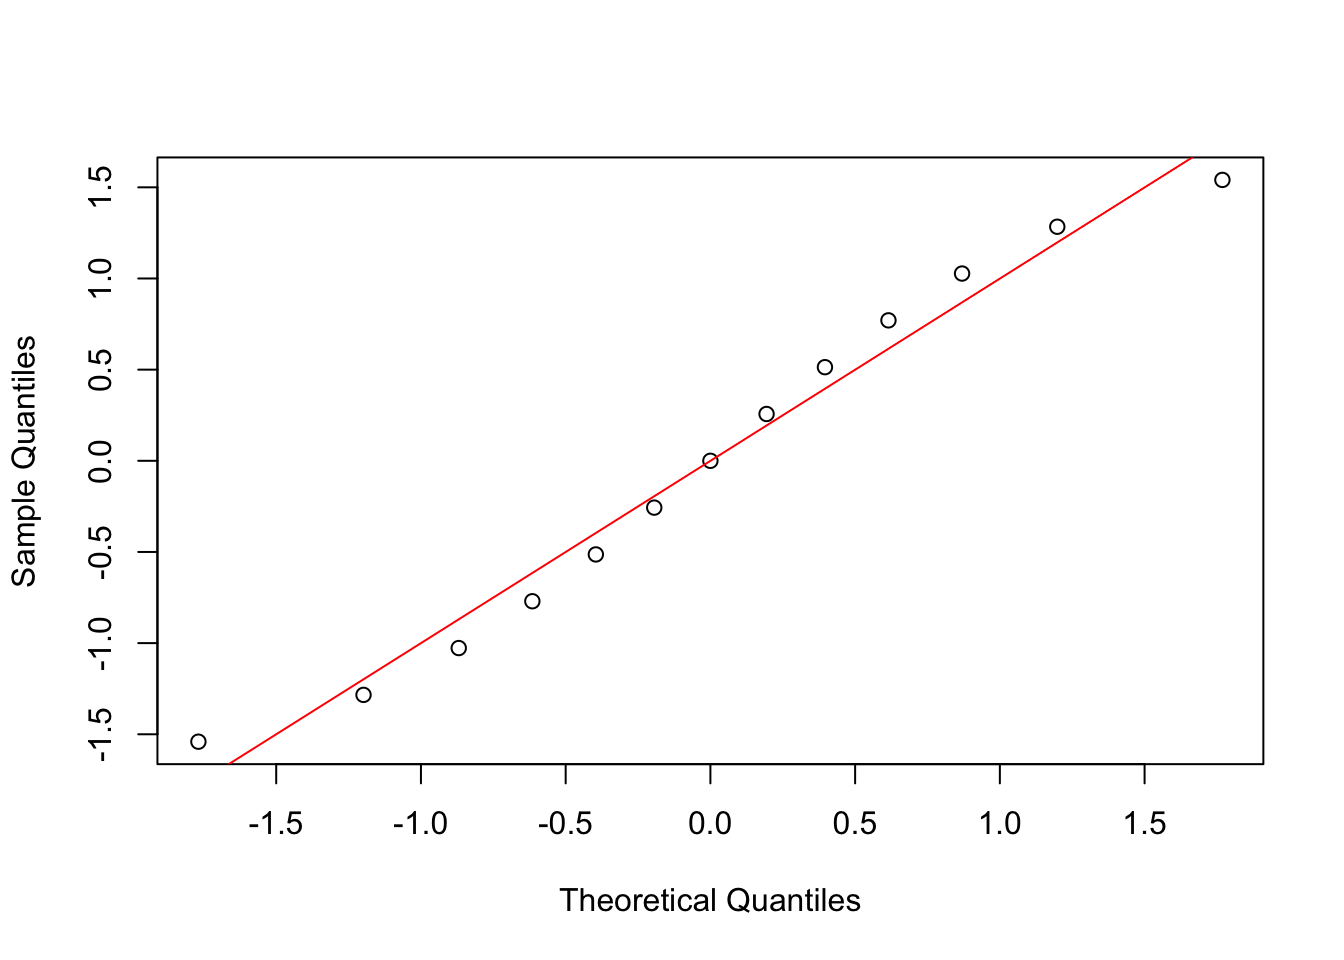
\includegraphics[width=0.2\textwidth]{../img/img13.png}}
\subfigure{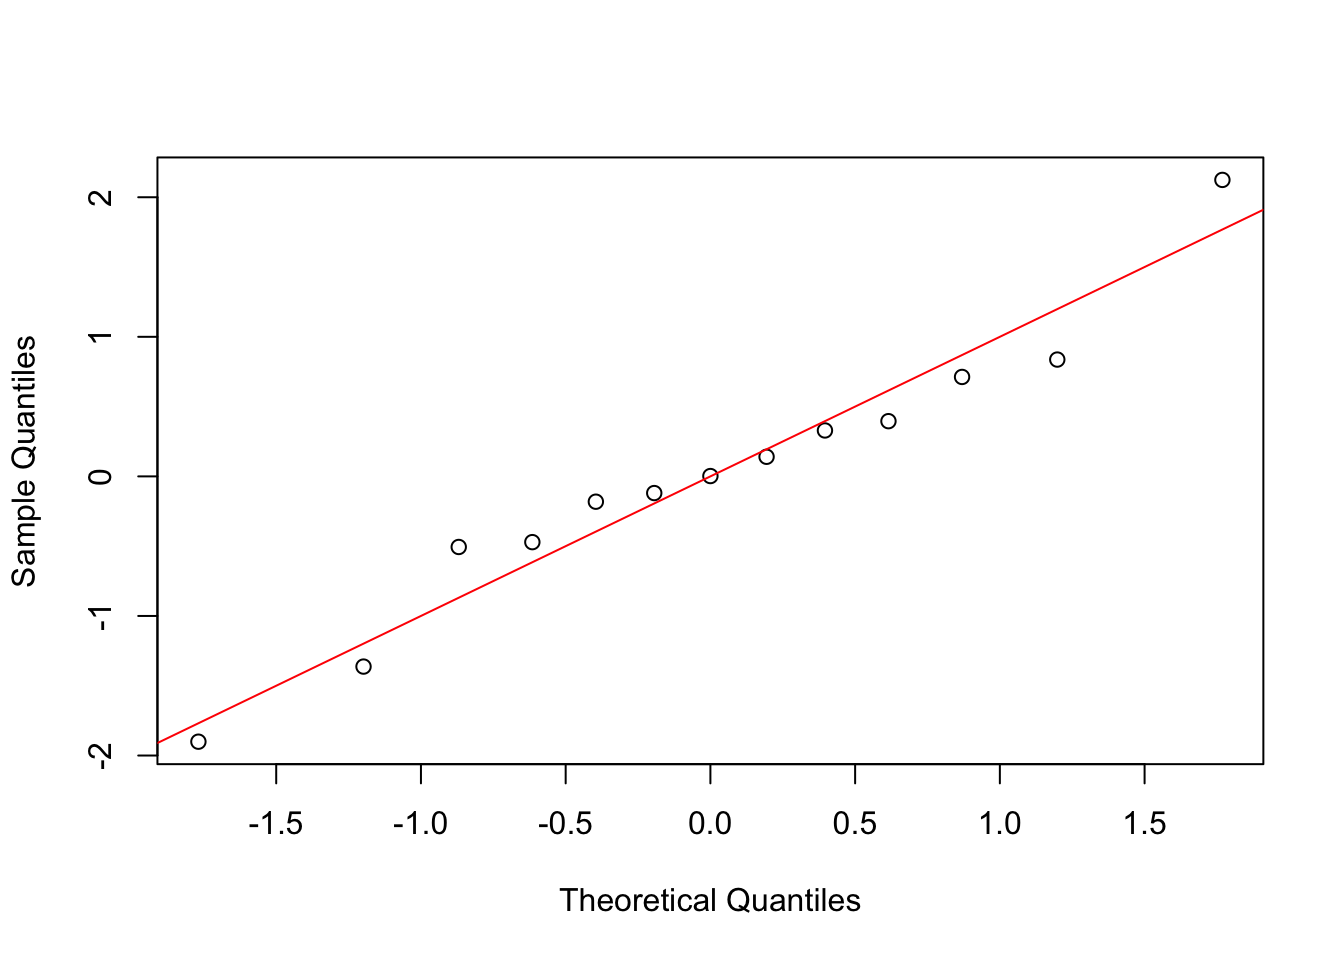
\includegraphics[width=0.2\textwidth]{../img/img14.png}}
\subfigure{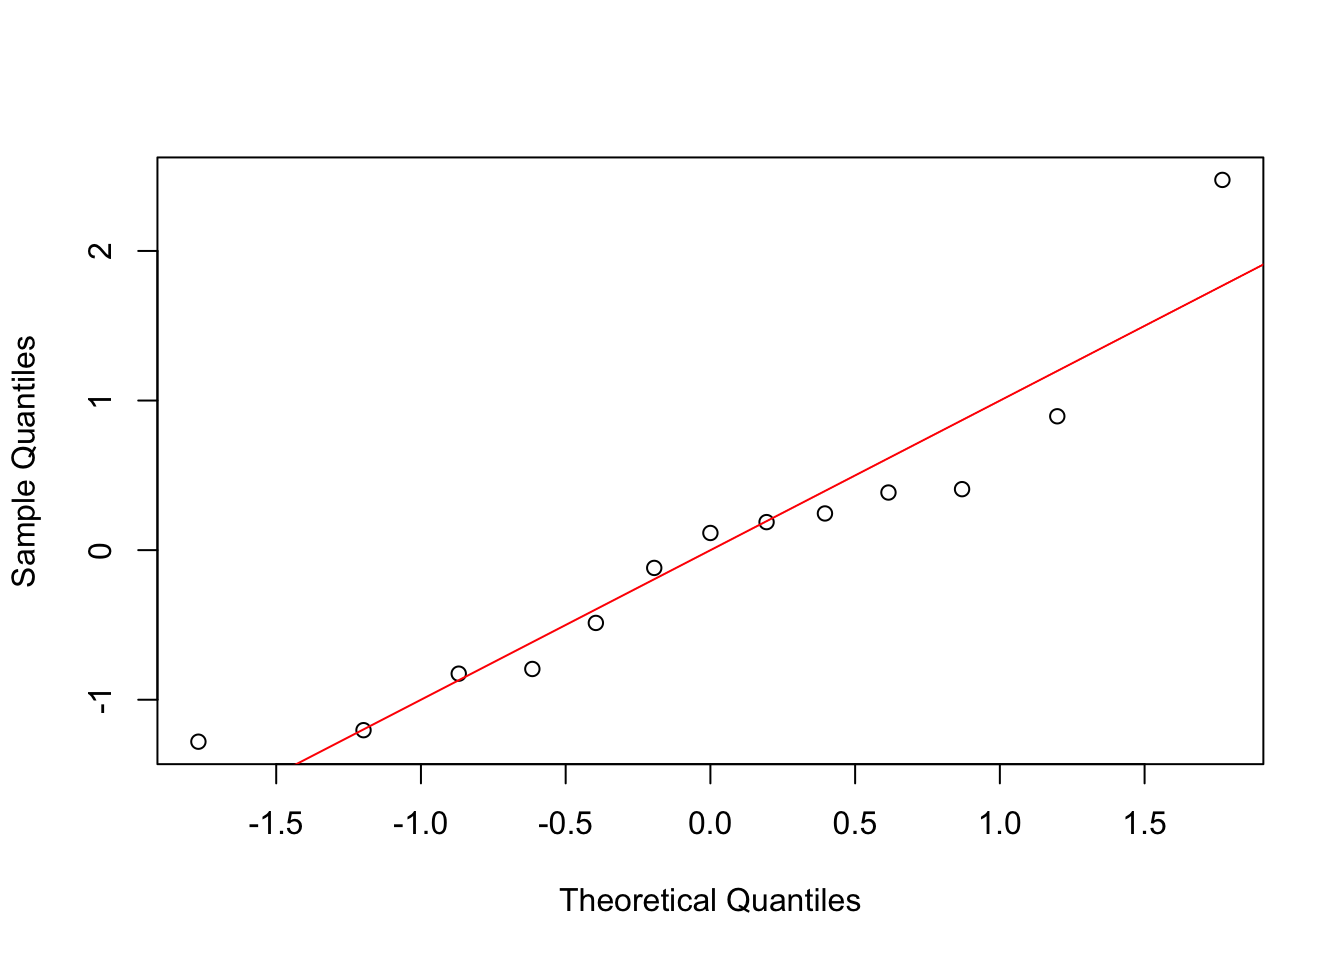
\includegraphics[width=0.2\textwidth]{../img/img15.png}}
\subfigure{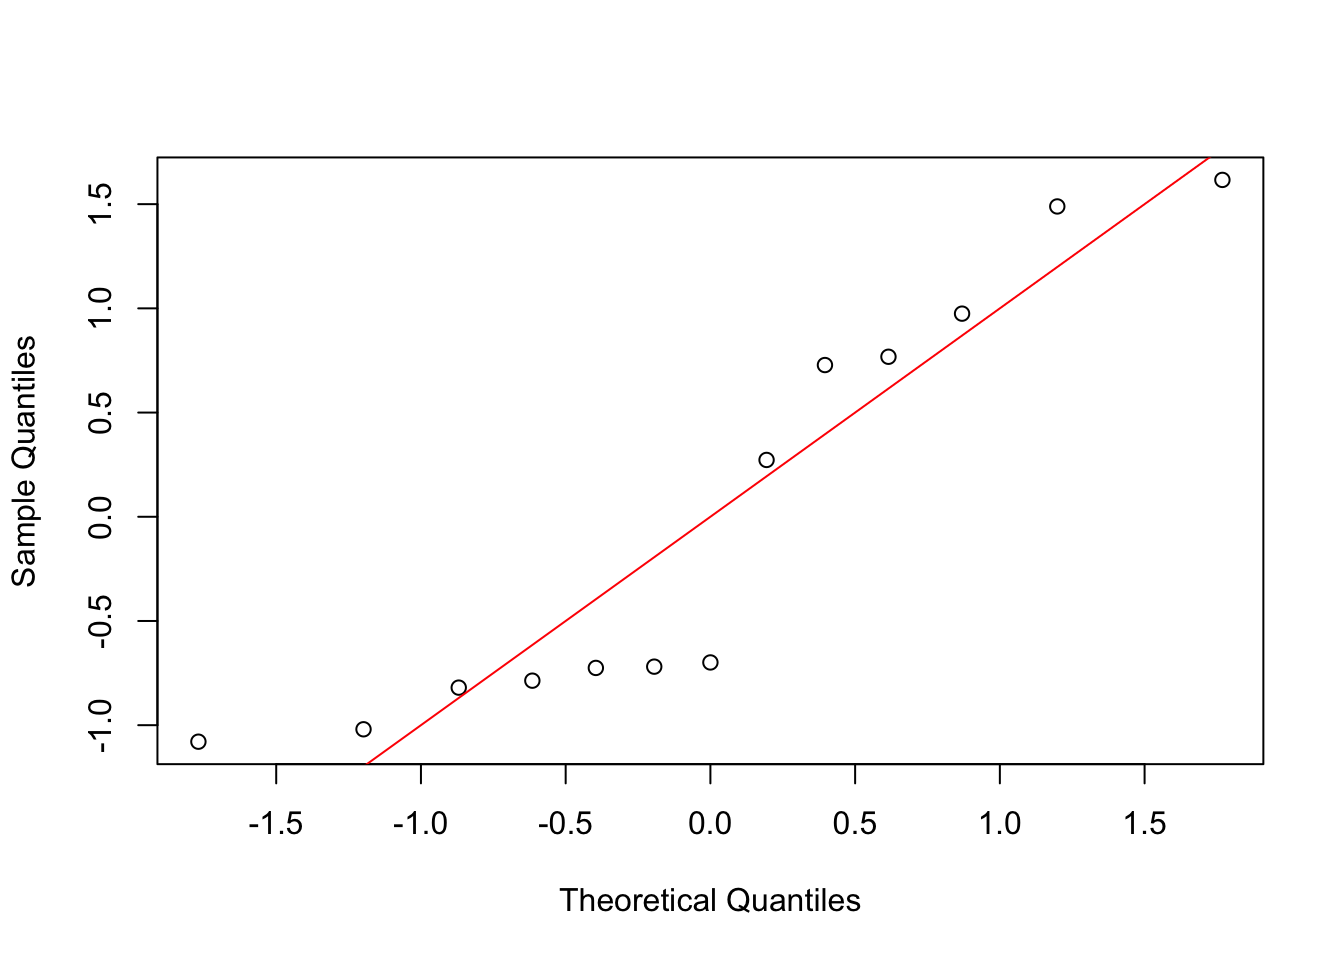
\includegraphics[width=0.2\textwidth]{../img/img16.png}}
\subfigure{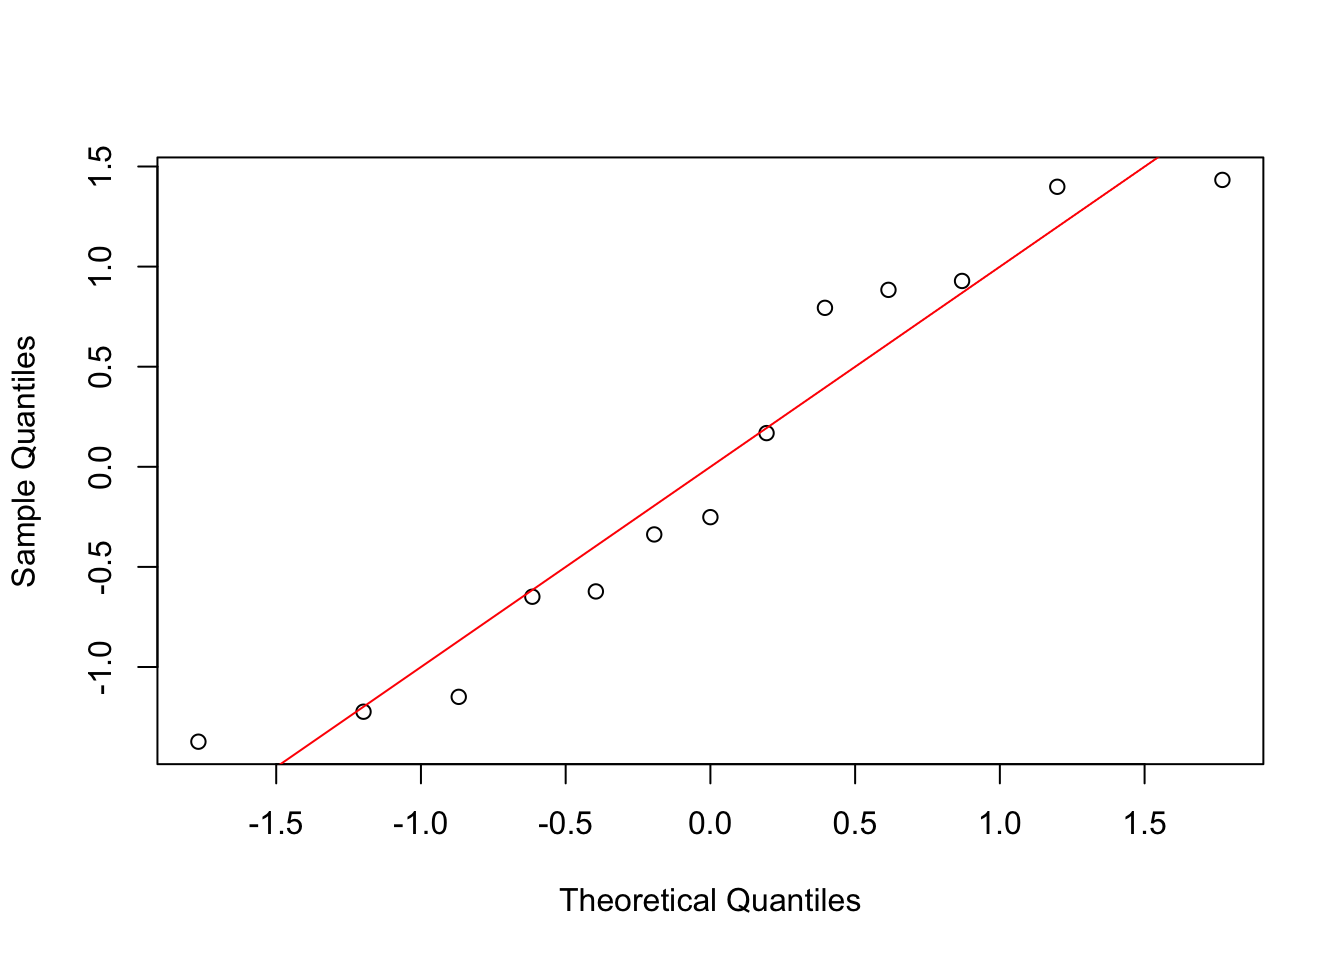
\includegraphics[width=0.2\textwidth]{../img/img17.png}}
\subfigure{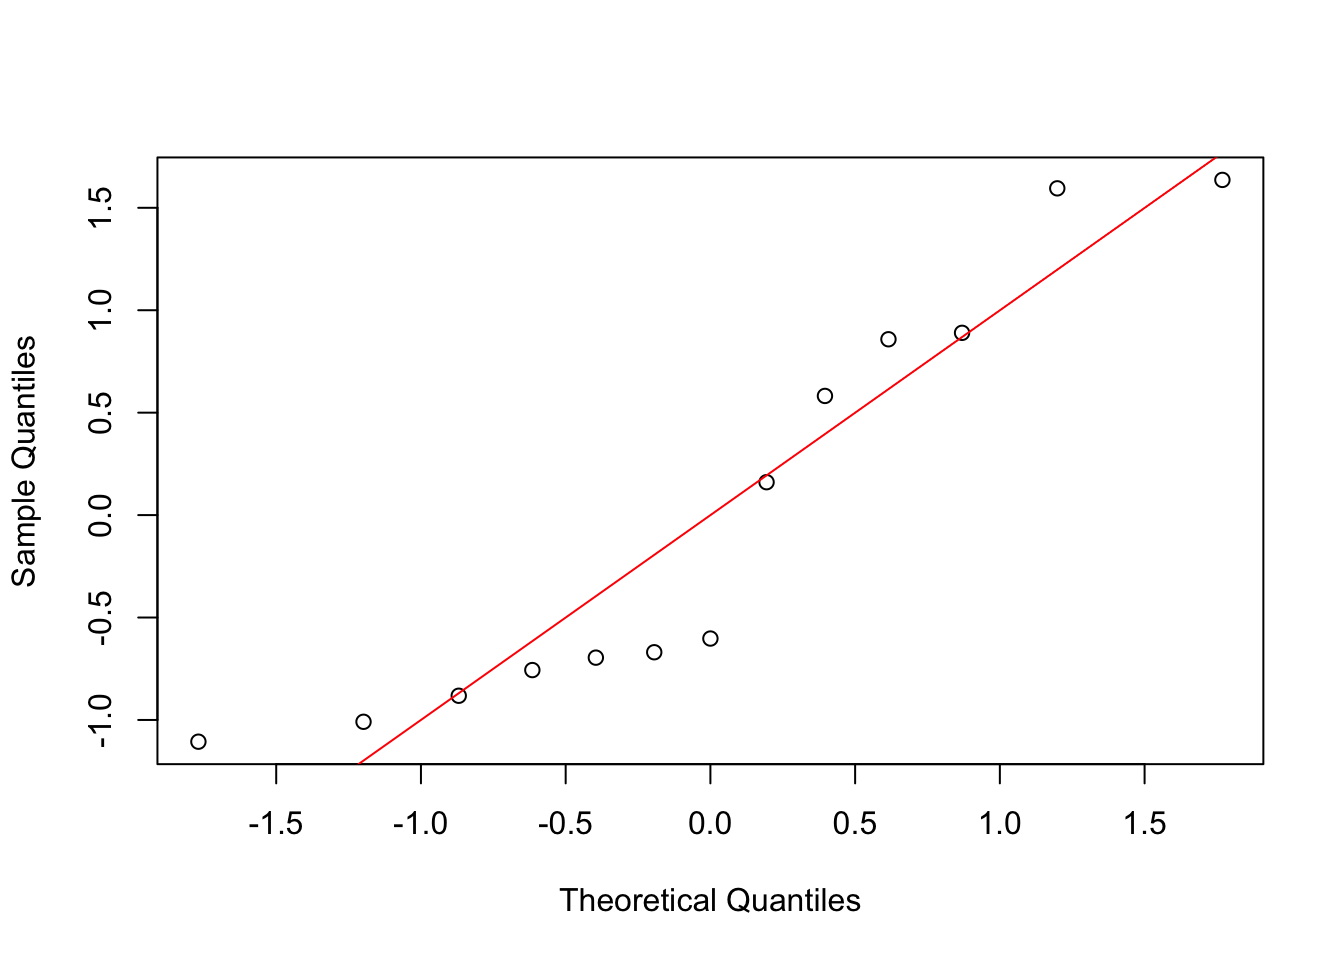
\includegraphics[width=0.2\textwidth]{../img/img18.png}}
\caption{Datos normalizados}
\end{figure}

Además del test de Shapiro–Wilk, que plantea la hipótesis nula que la muestra proviene de una distribución normal, de donde obtenemos la normalidad para todos los datos menos \emph{x6} y \emph{x8}.

\subsection{Análisis exploratorio multivariante}

Comenzamos realizando un test de Bartlett para estudiar la correlación entre las variables, con el cuál obtenemos un \emph{p-valor} pequeño, lo que nos indica que, en efecto están correladas, lo que nos permite realizar el Análisis de Componentes Principales (ACP).

Para ello, visualizamos la varianza explicada y acumulada por cada componente:
\begin{figure}[H]
\centering
\subfigure{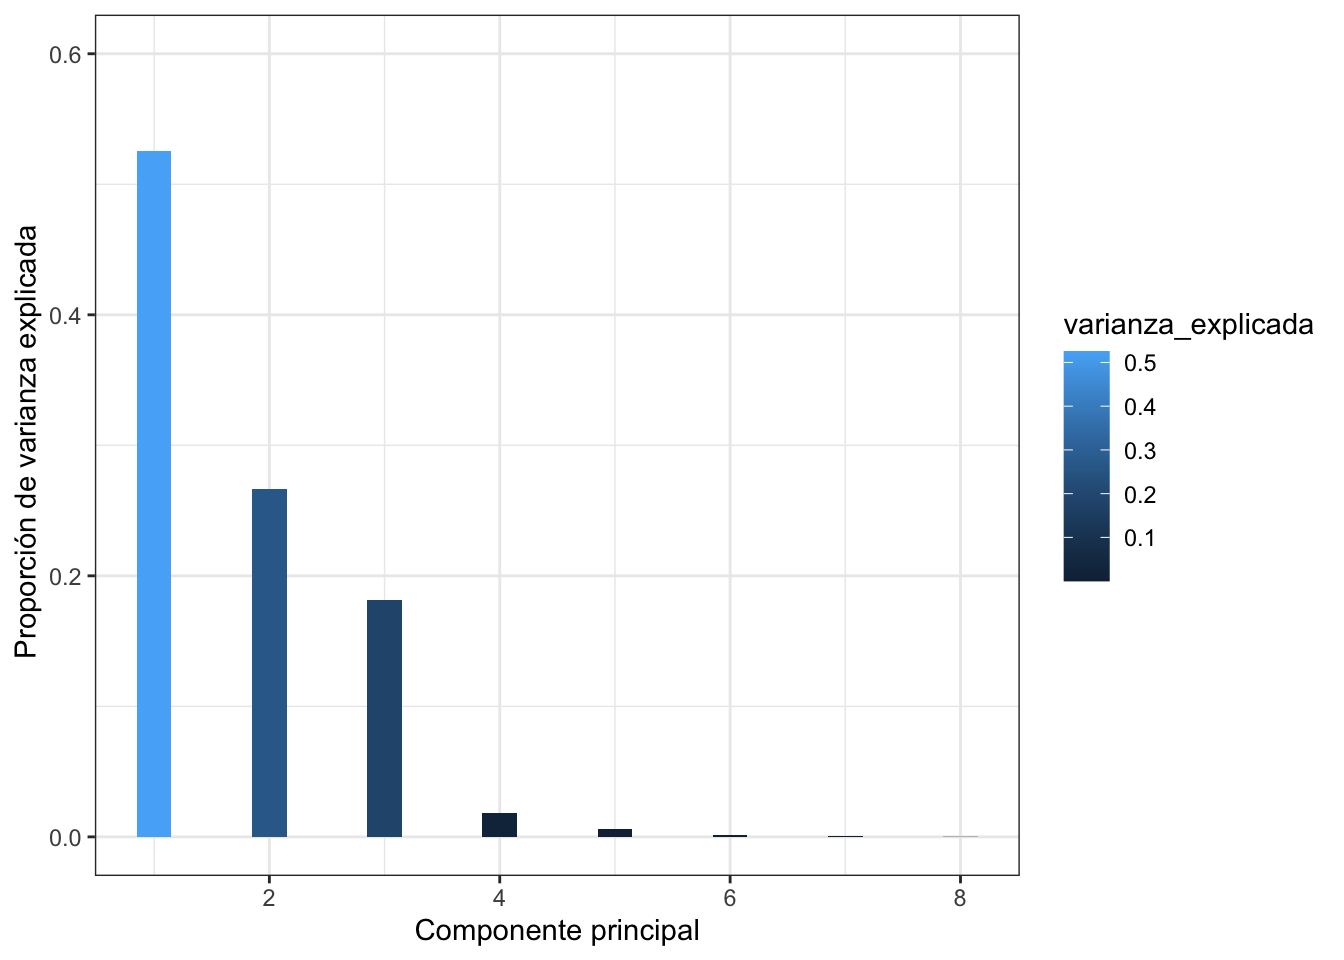
\includegraphics[width=0.4\textwidth]{../img/img19.png}}
\subfigure{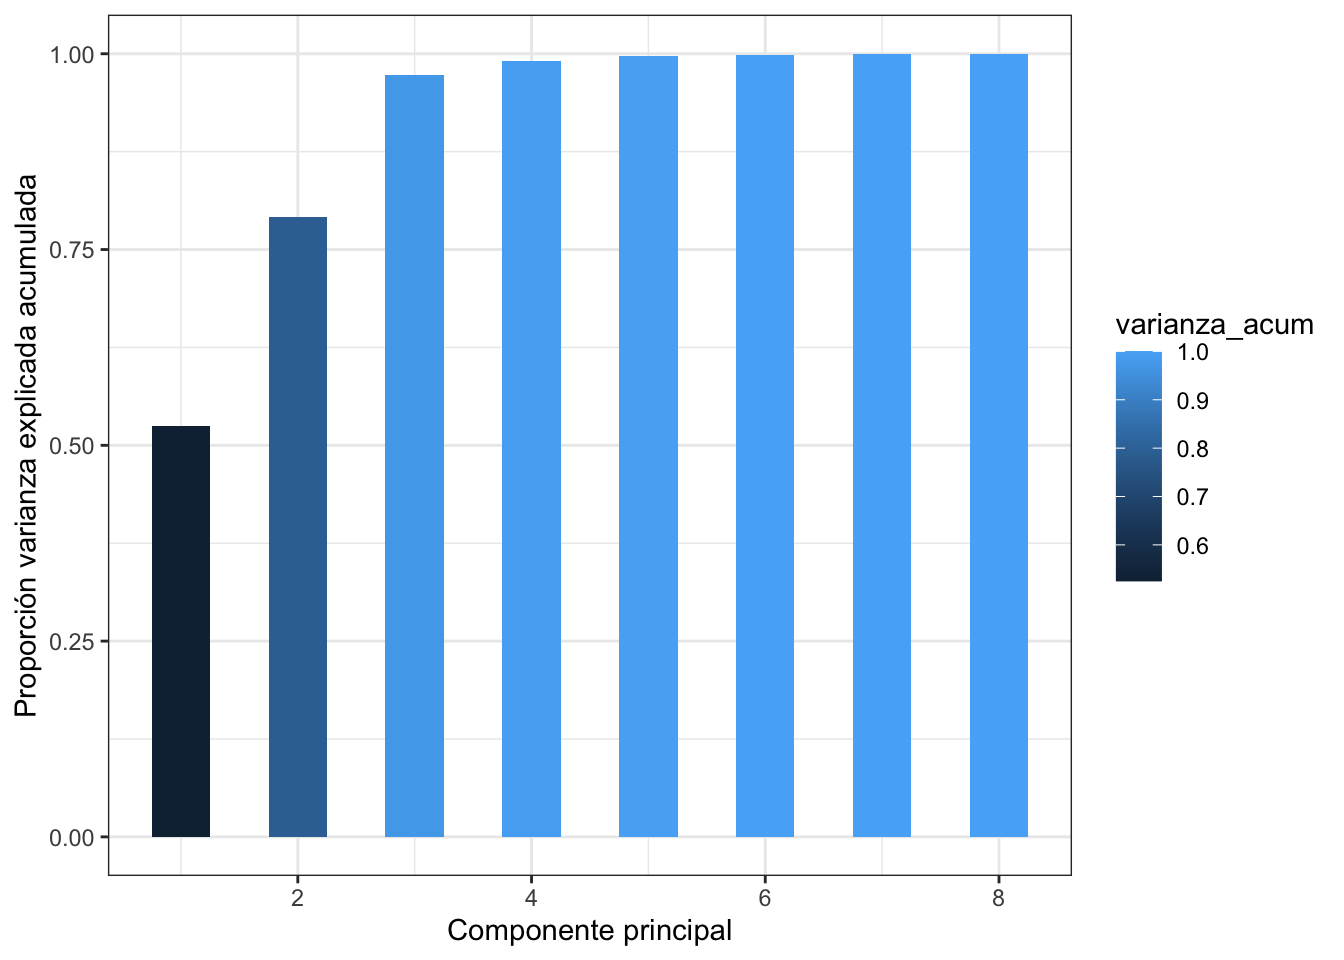
\includegraphics[width=0.4\textwidth]{../img/img20.png}}
\end{figure}

Con esto, y utilizando el método del codo, que nos da la siguiente gráfica:
\begin{figure}[H]
\centering
\subfigure{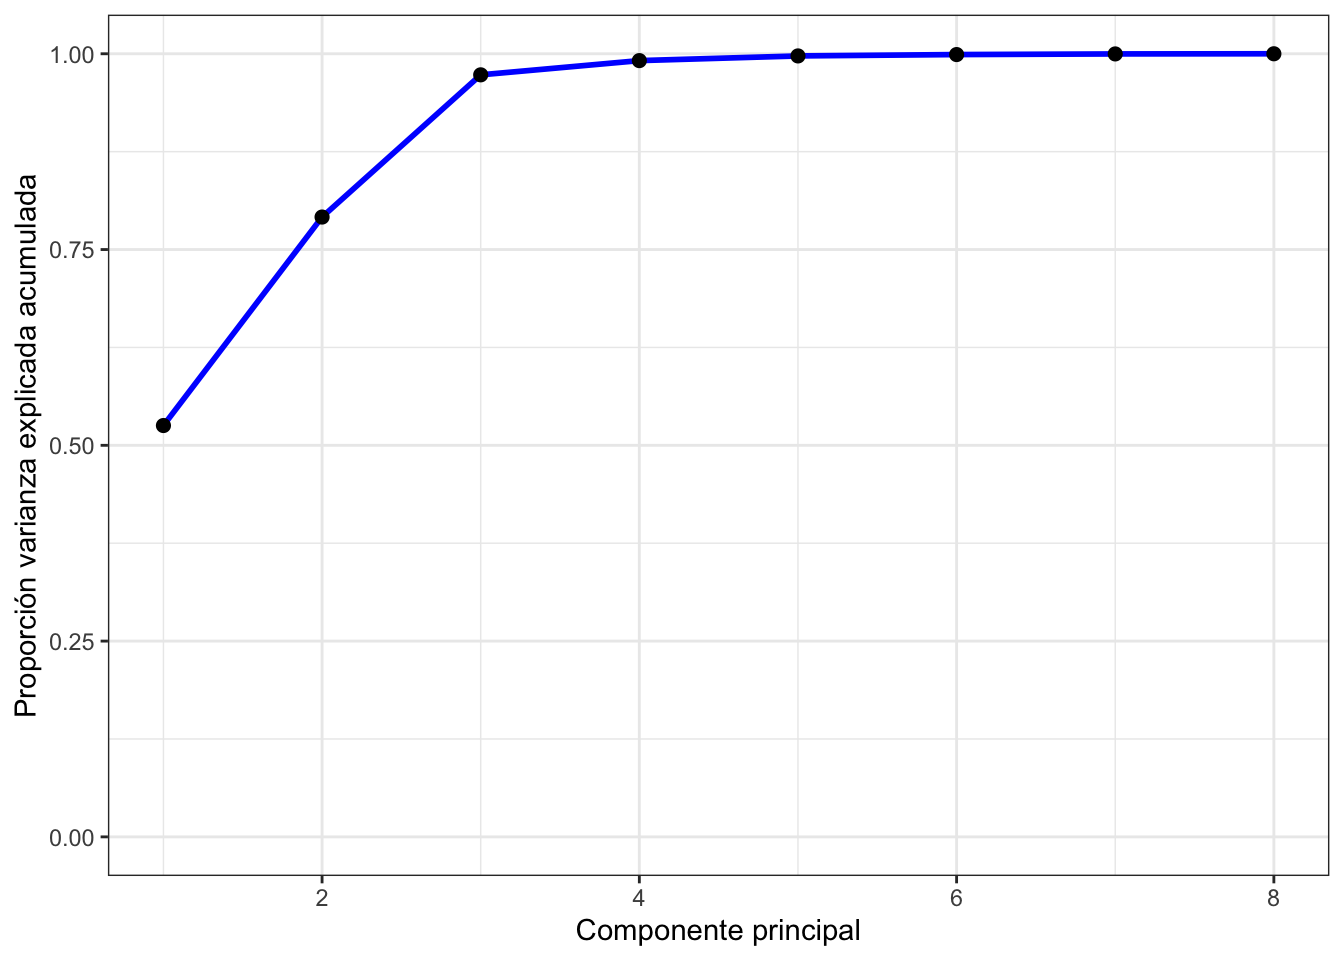
\includegraphics[width=0.5\textwidth]{../img/img21.png}}
\end{figure}
tenemos que el número de componentes óptimo para reducir la dimensionalidad es 3.

Se visualiza la contribución de cada componente en las siguientes gráficas:
\begin{figure}[H]
\centering
\subfigure{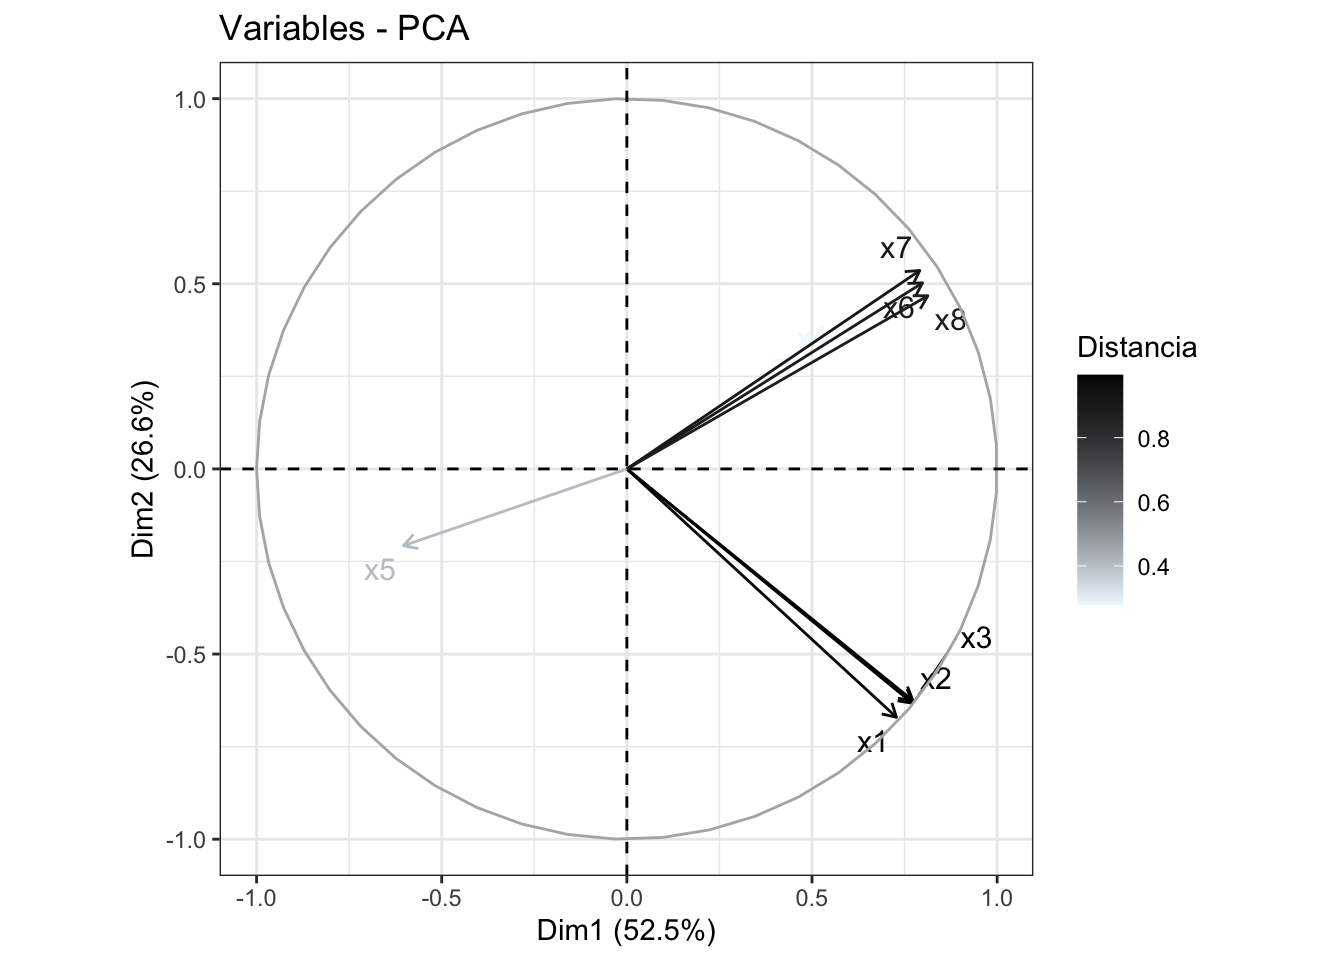
\includegraphics[width=0.3\textwidth]{../img/img22.png}}
\subfigure{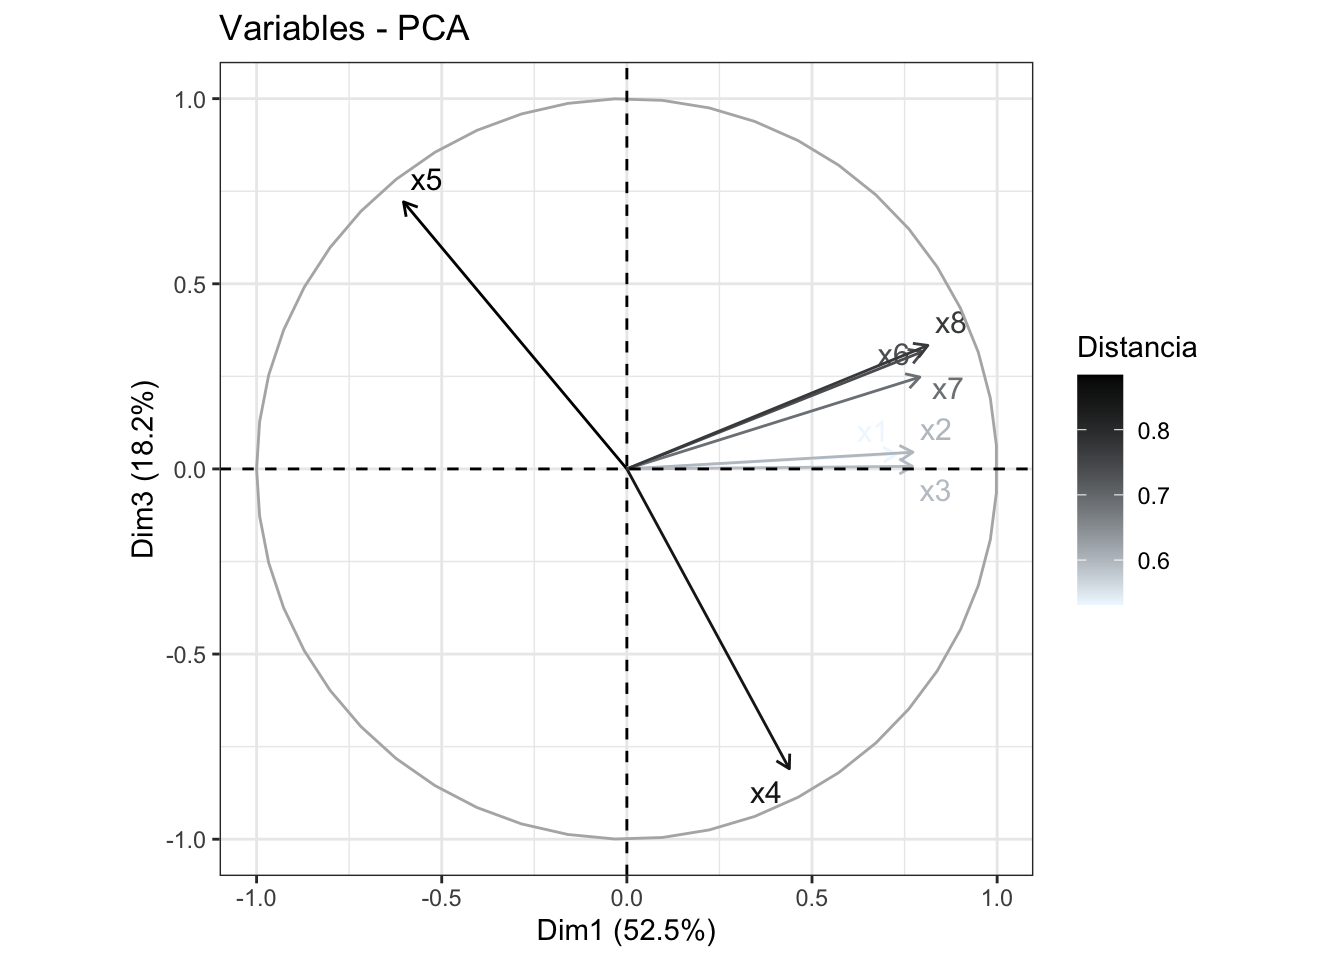
\includegraphics[width=0.3\textwidth]{../img/img23.png}}
\subfigure{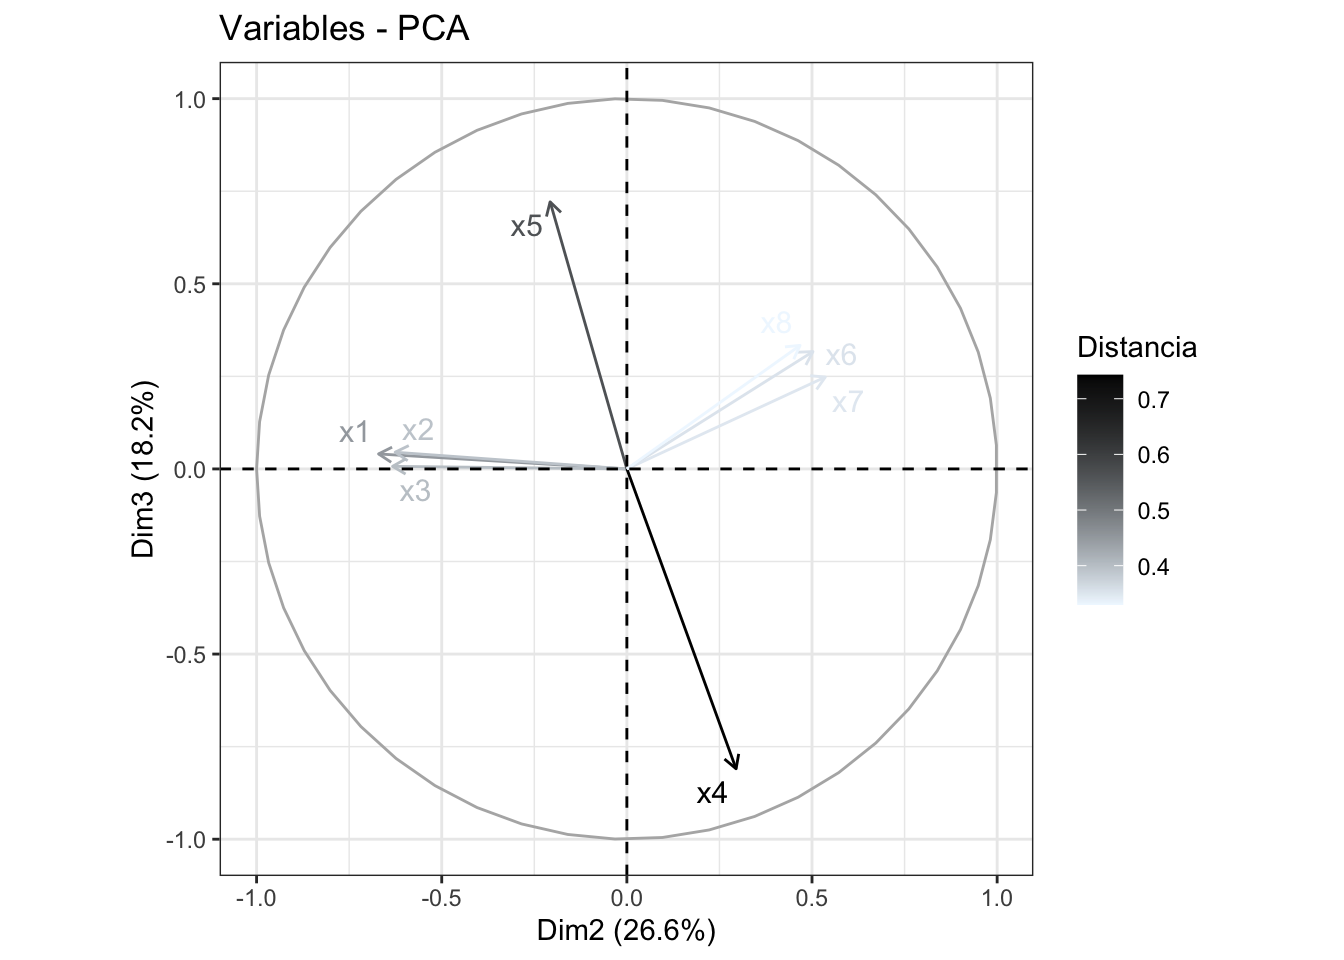
\includegraphics[width=0.3\textwidth]{../img/img24.png}}
\end{figure}

\begin{figure}[H]
\centering
\subfigure{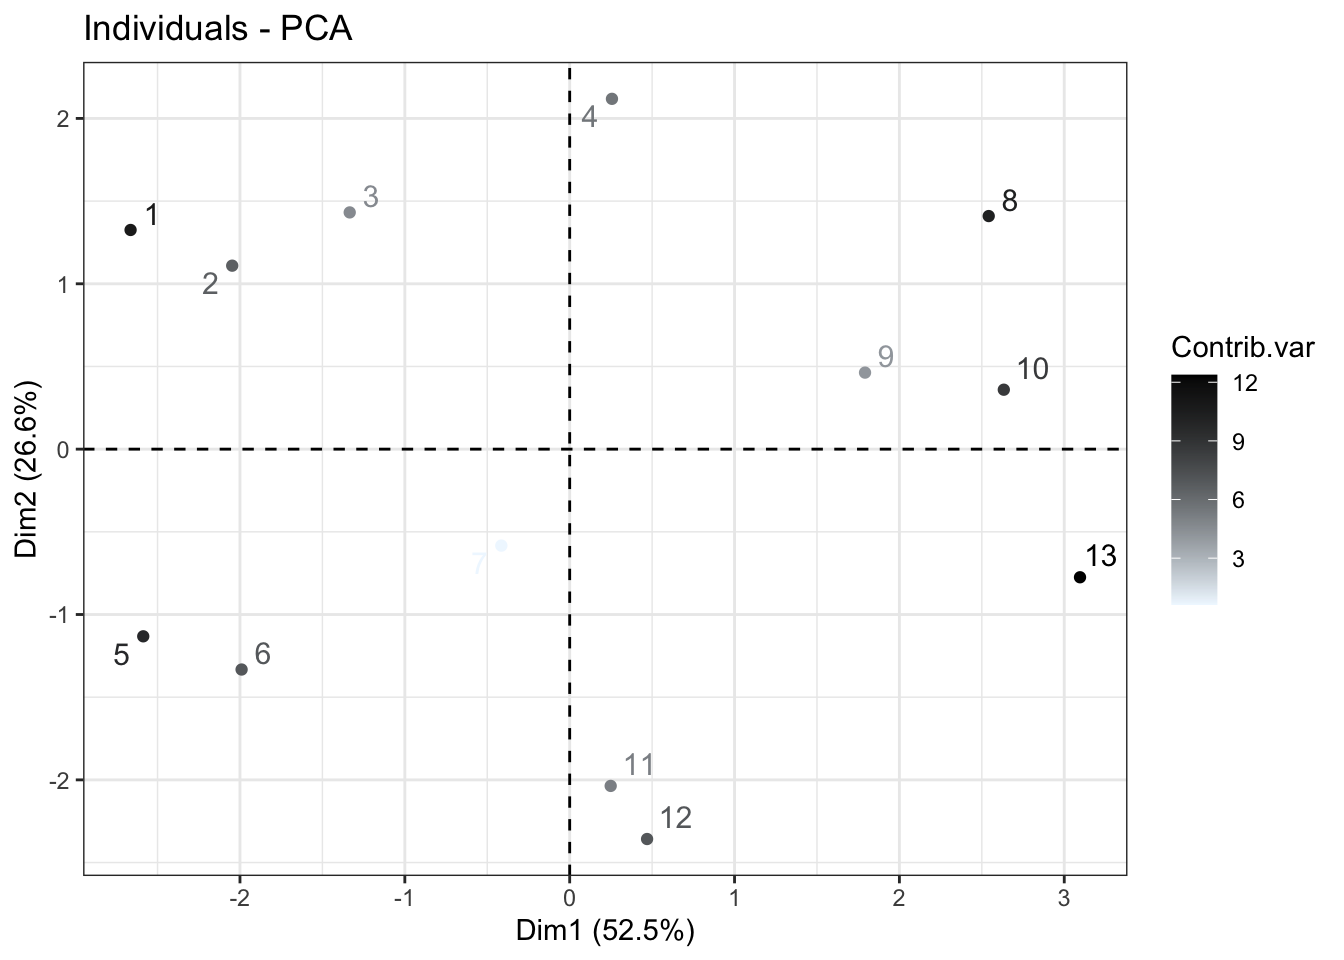
\includegraphics[width=0.3\textwidth]{../img/img25.png}}
\subfigure{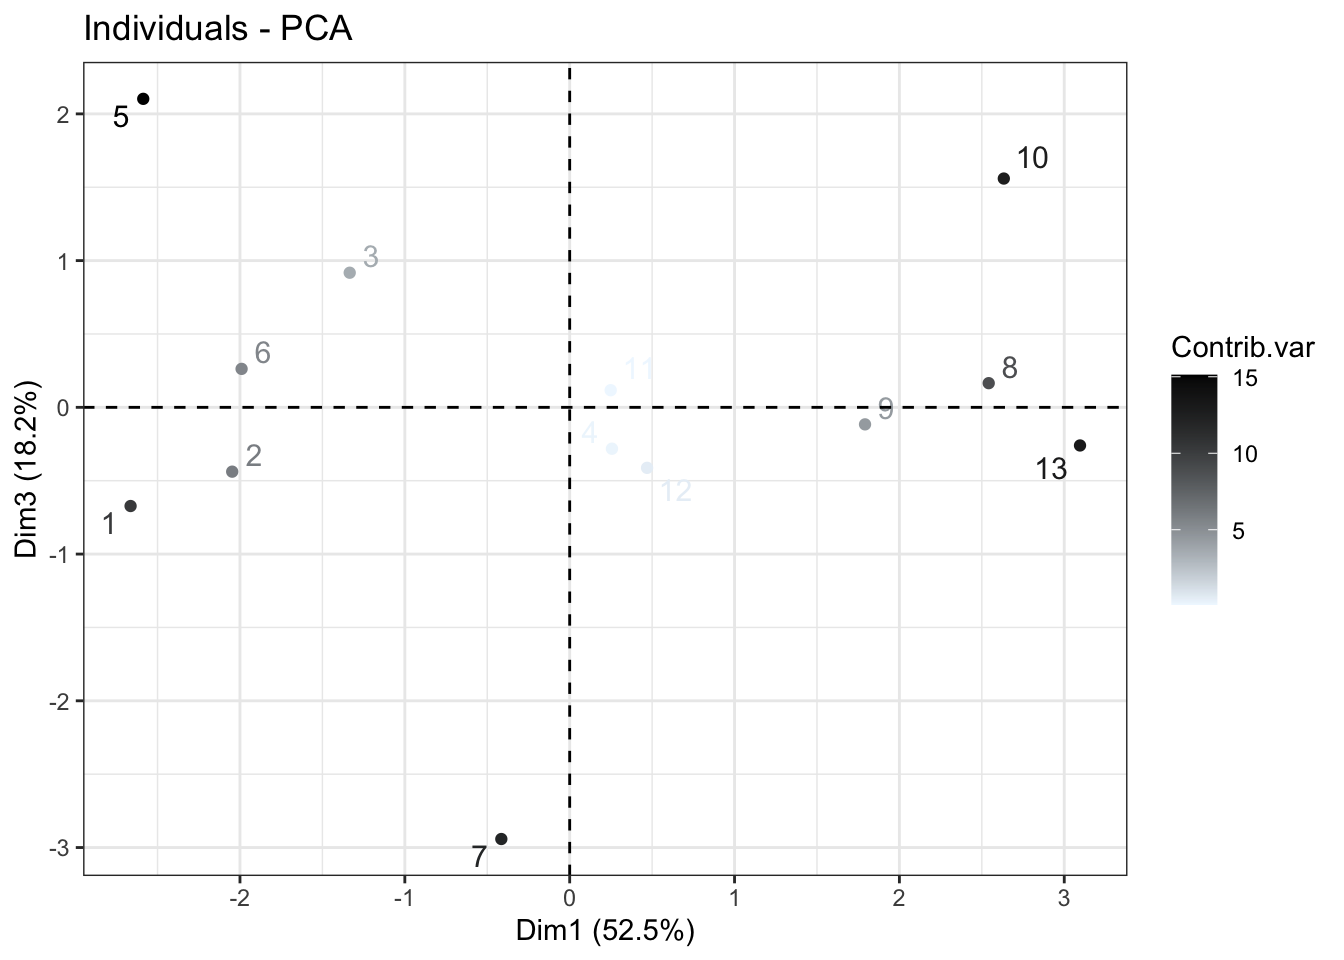
\includegraphics[width=0.3\textwidth]{../img/img26.png}}
\subfigure{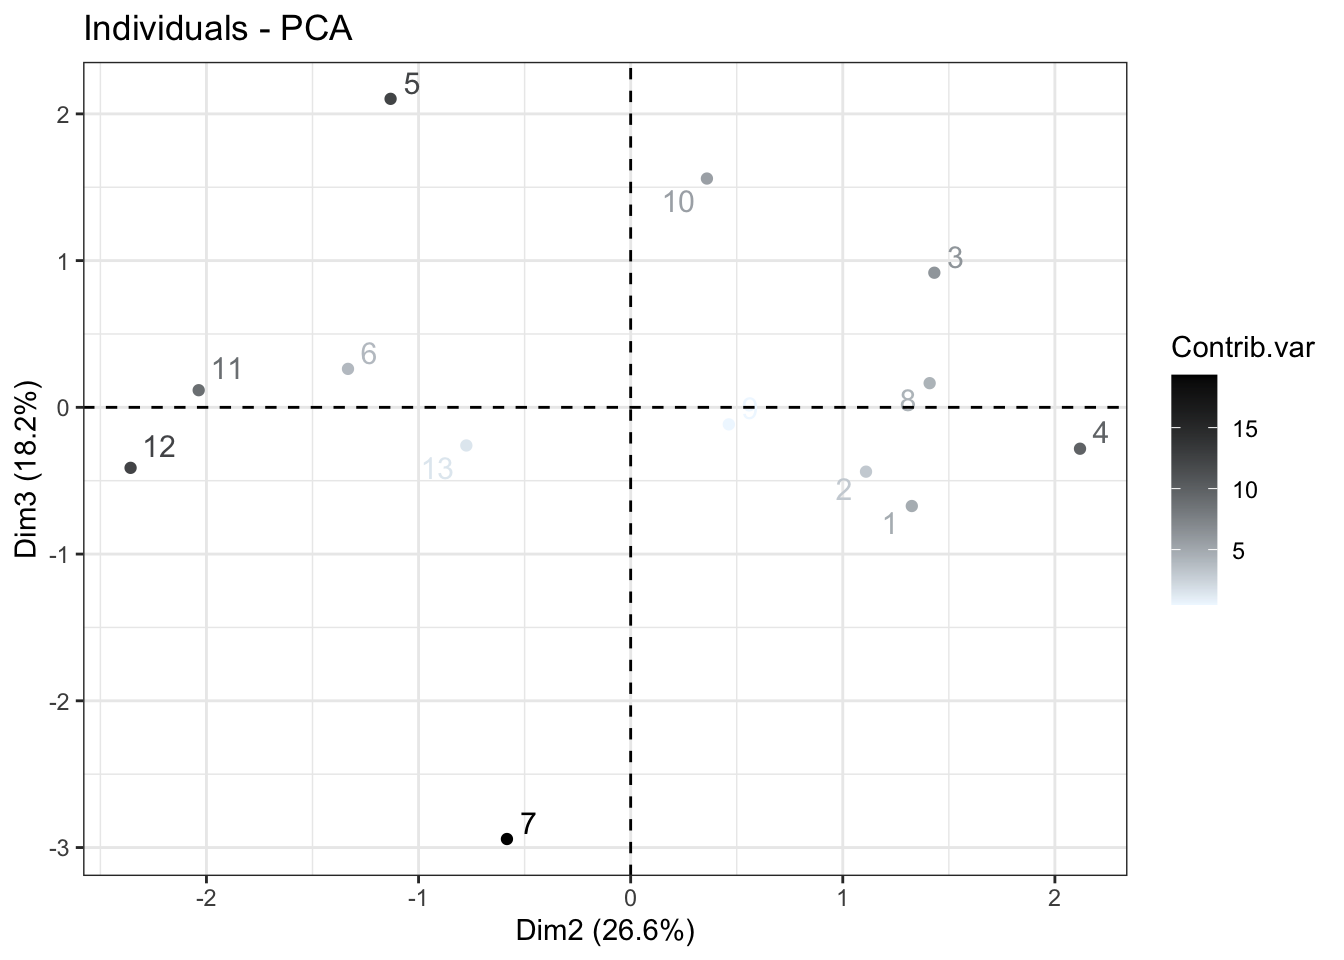
\includegraphics[width=0.3\textwidth]{../img/img27.png}}
\end{figure}

\begin{figure}[H]
\centering
\subfigure{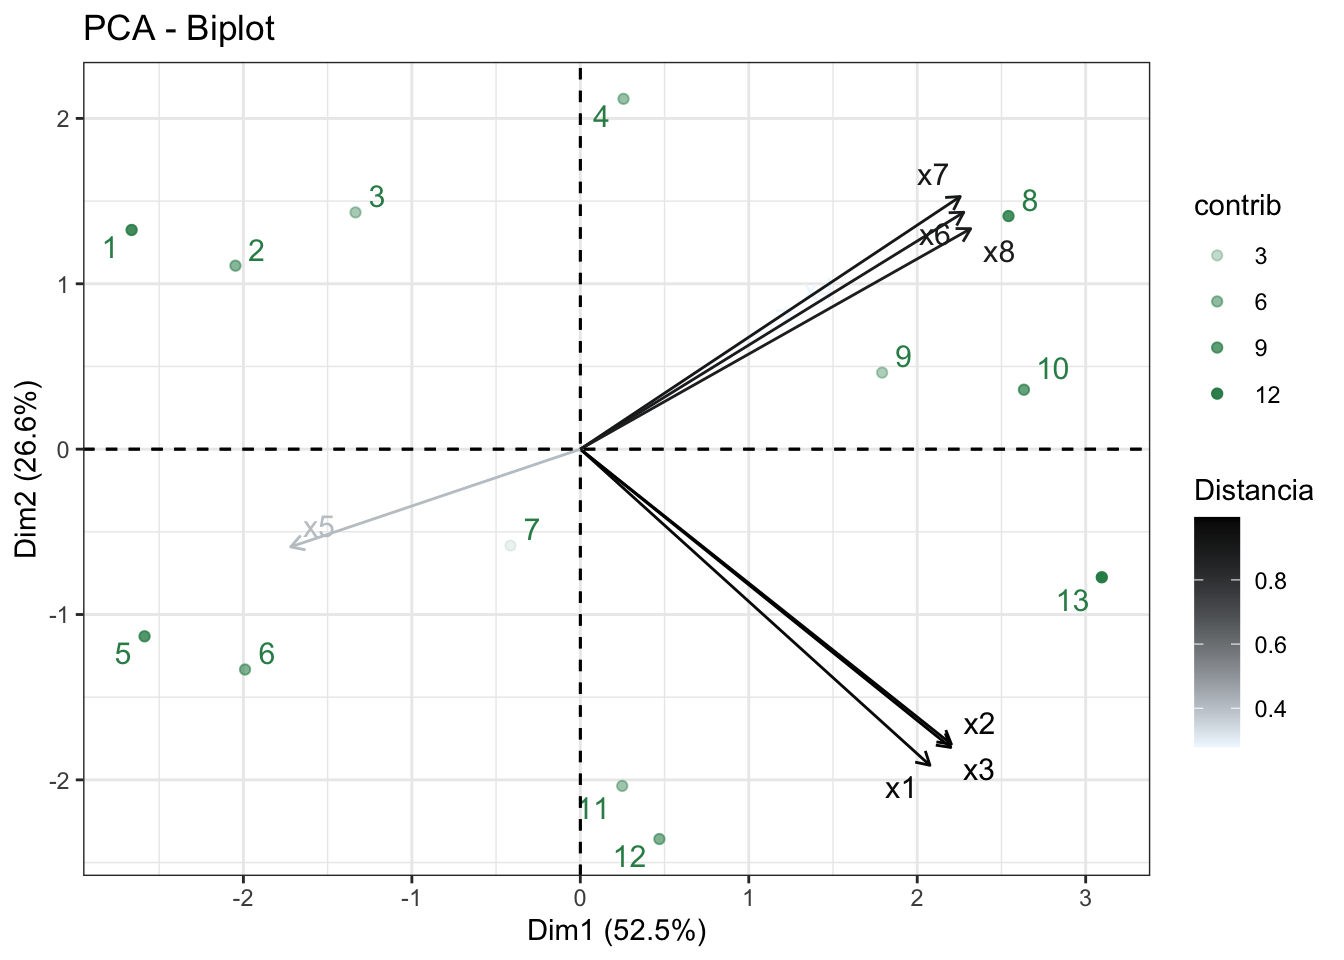
\includegraphics[width=0.3\textwidth]{../img/img28.png}}
\subfigure{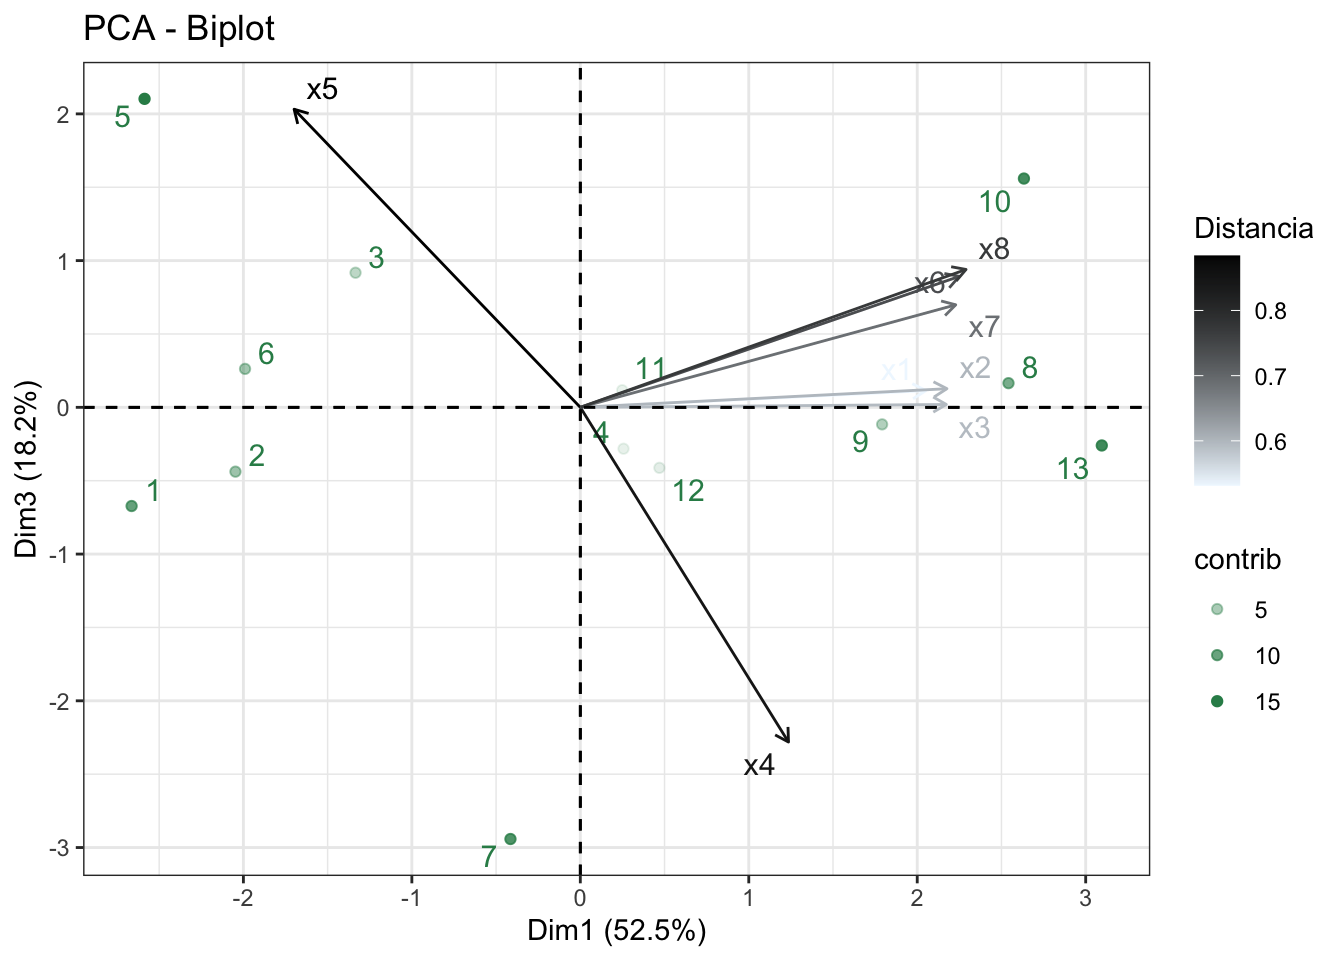
\includegraphics[width=0.3\textwidth]{../img/img29.png}}
\subfigure{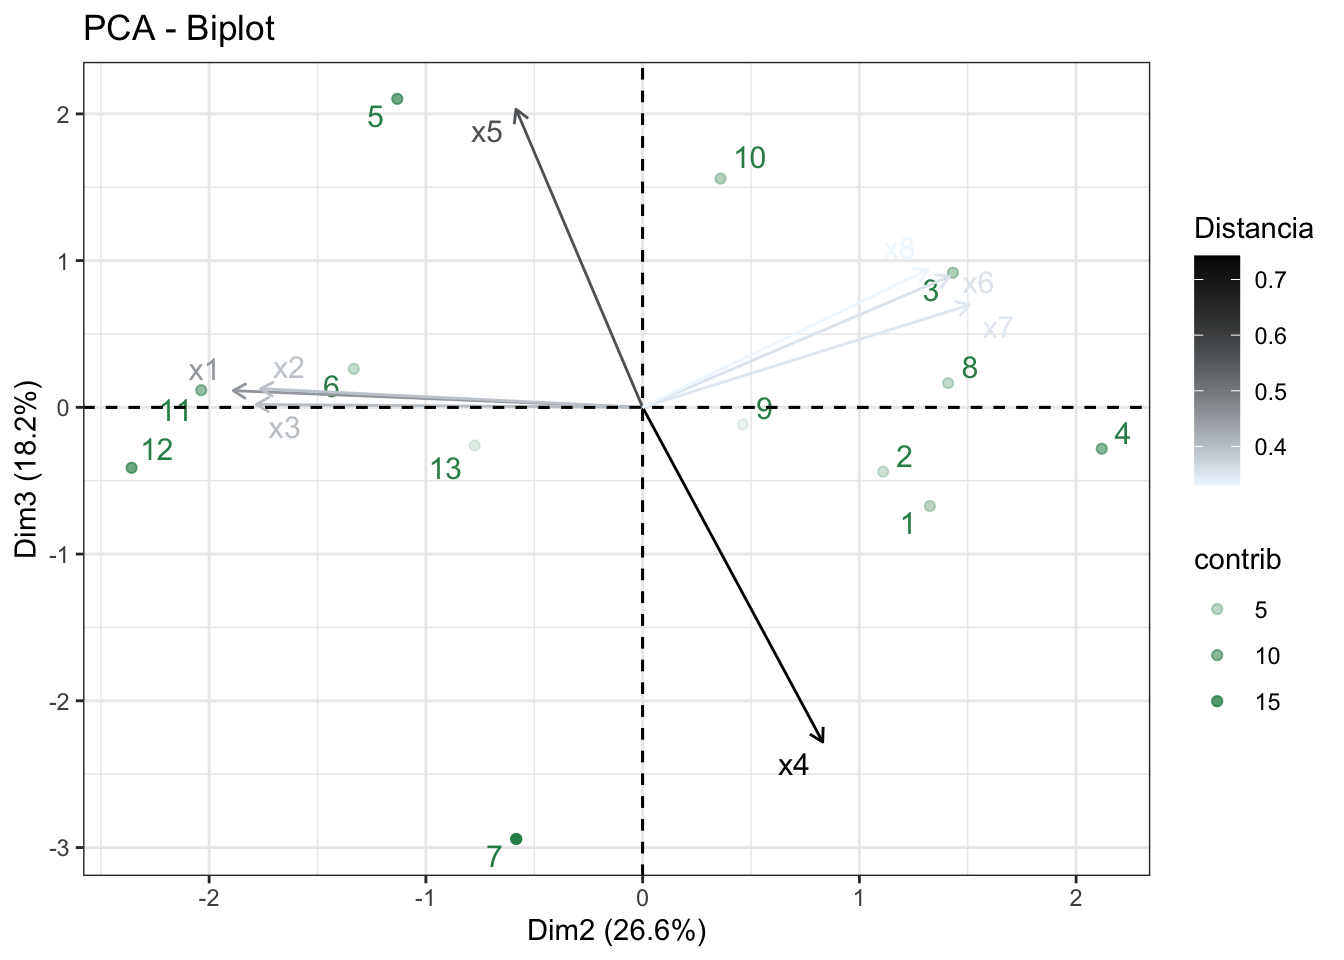
\includegraphics[width=0.3\textwidth]{../img/img30.png}}
\end{figure}

Para el Análisis Factorial (AF) comenzamos visualizando las correlaciones:
\begin{figure}[H]
\centering
\subfigure{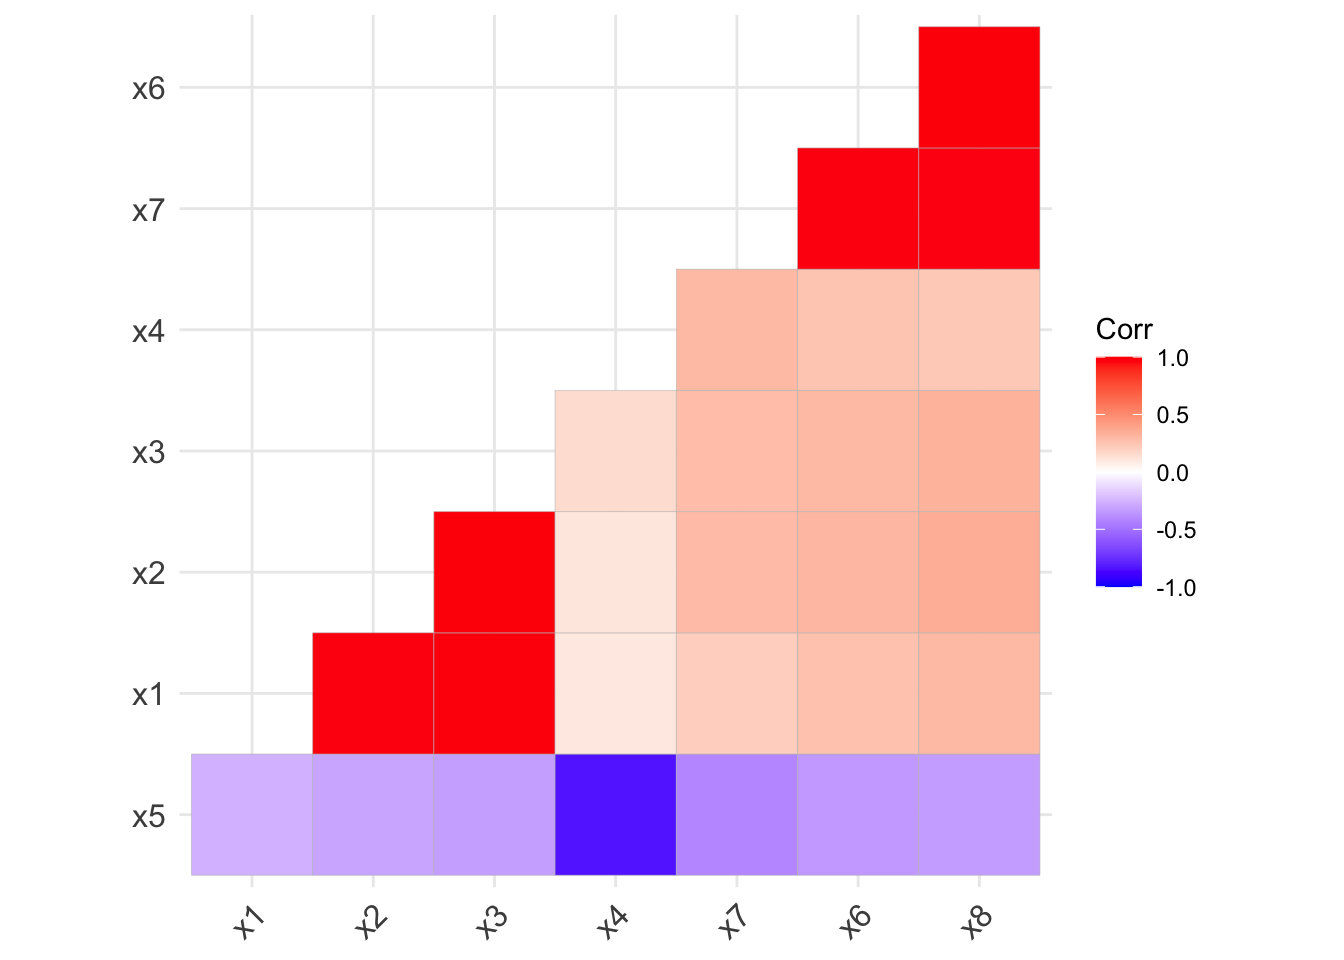
\includegraphics[width=0.4\textwidth]{../img/img31.png}}
\subfigure{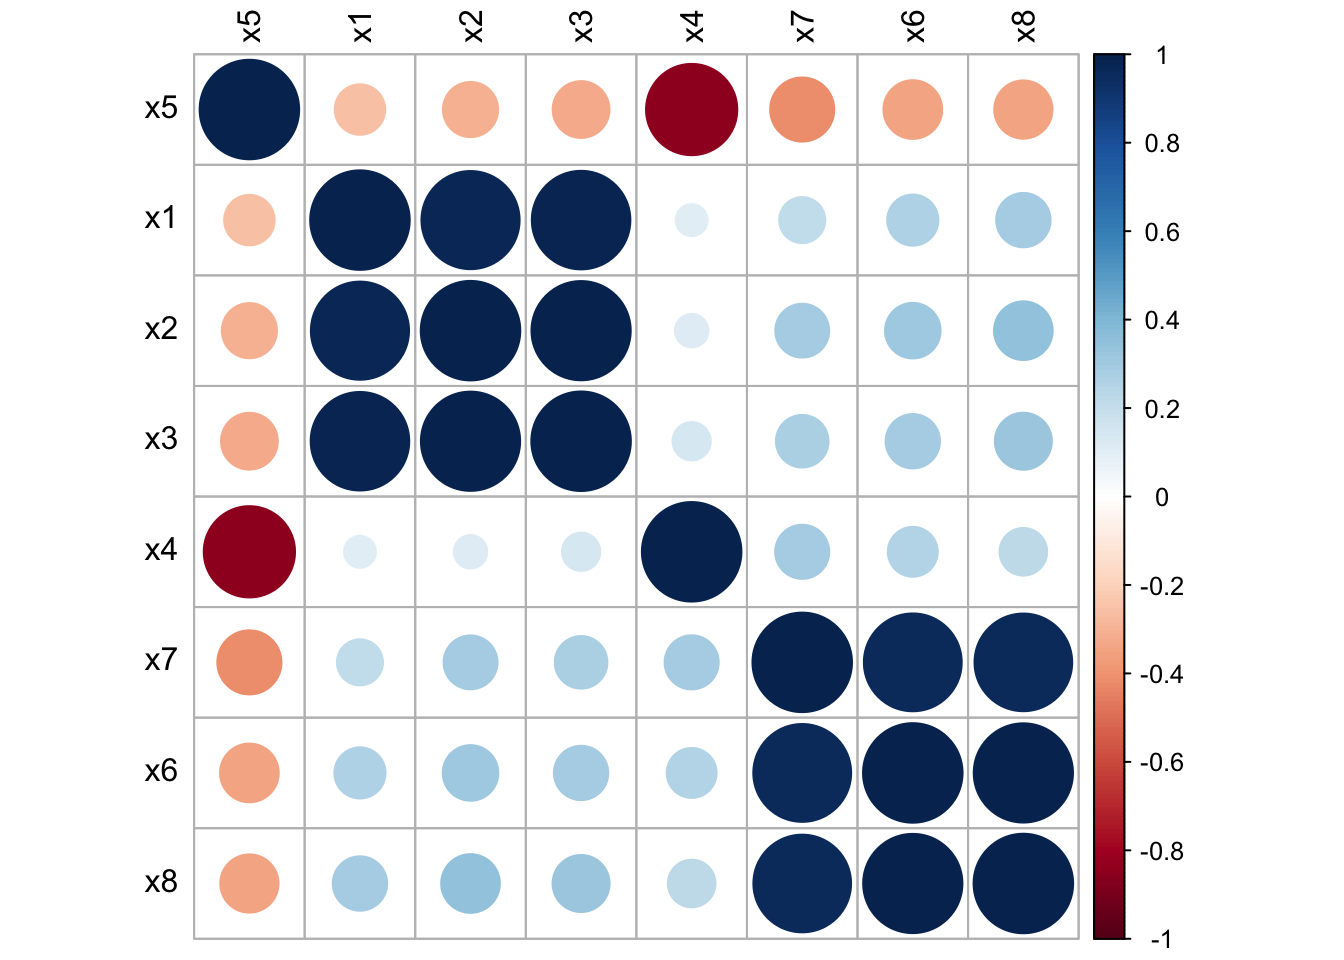
\includegraphics[width=0.4\textwidth]{../img/img32.png}}
\end{figure}

Para decidir el número de factores, utilizamos los siguientes gráficos:
\begin{figure}[H]
\centering
\subfigure{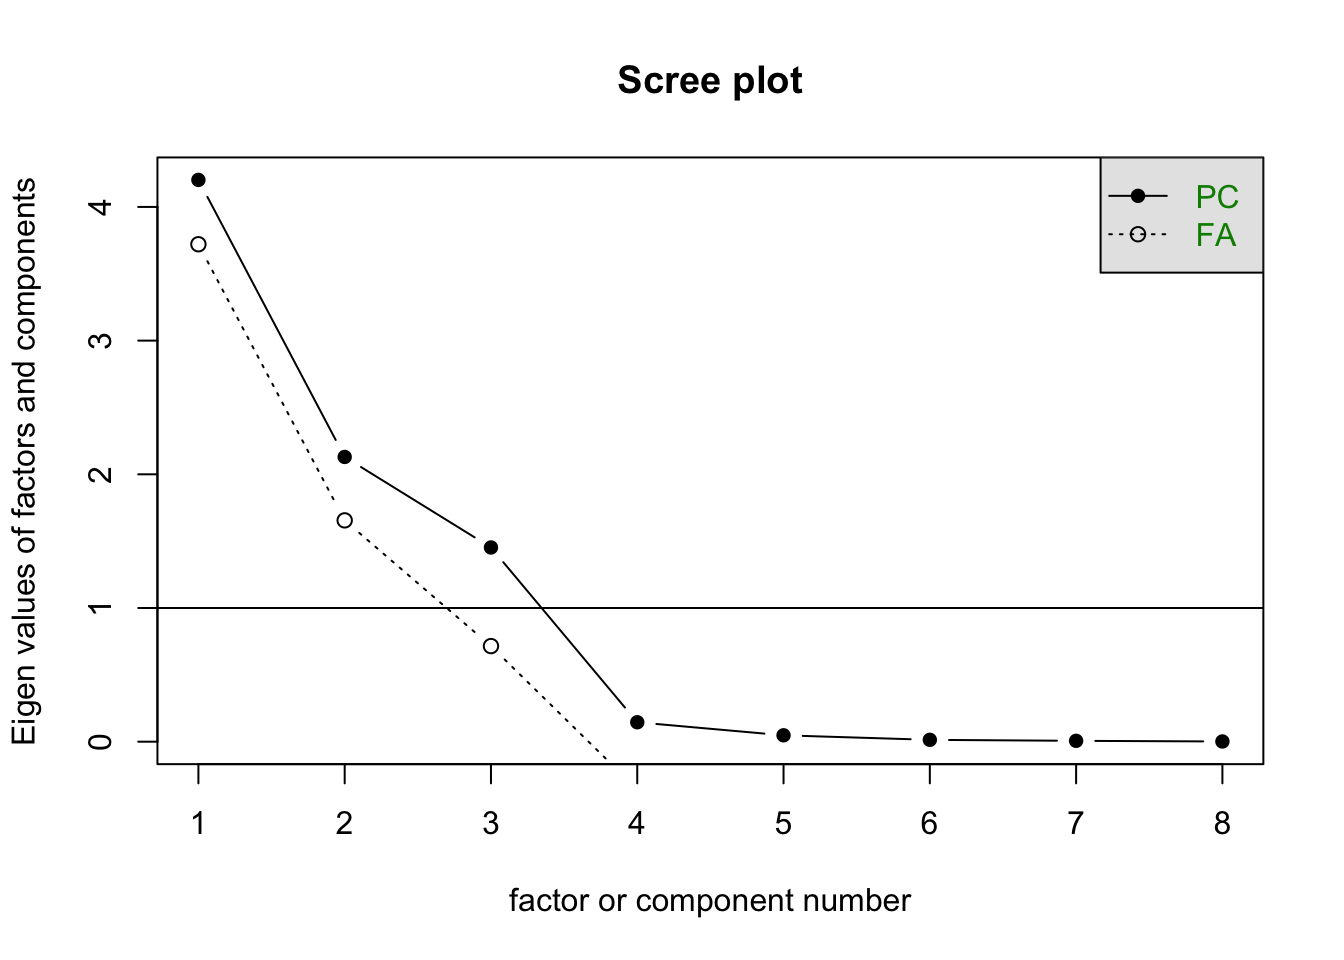
\includegraphics[width=0.4\textwidth]{../img/img33.png}}
\subfigure{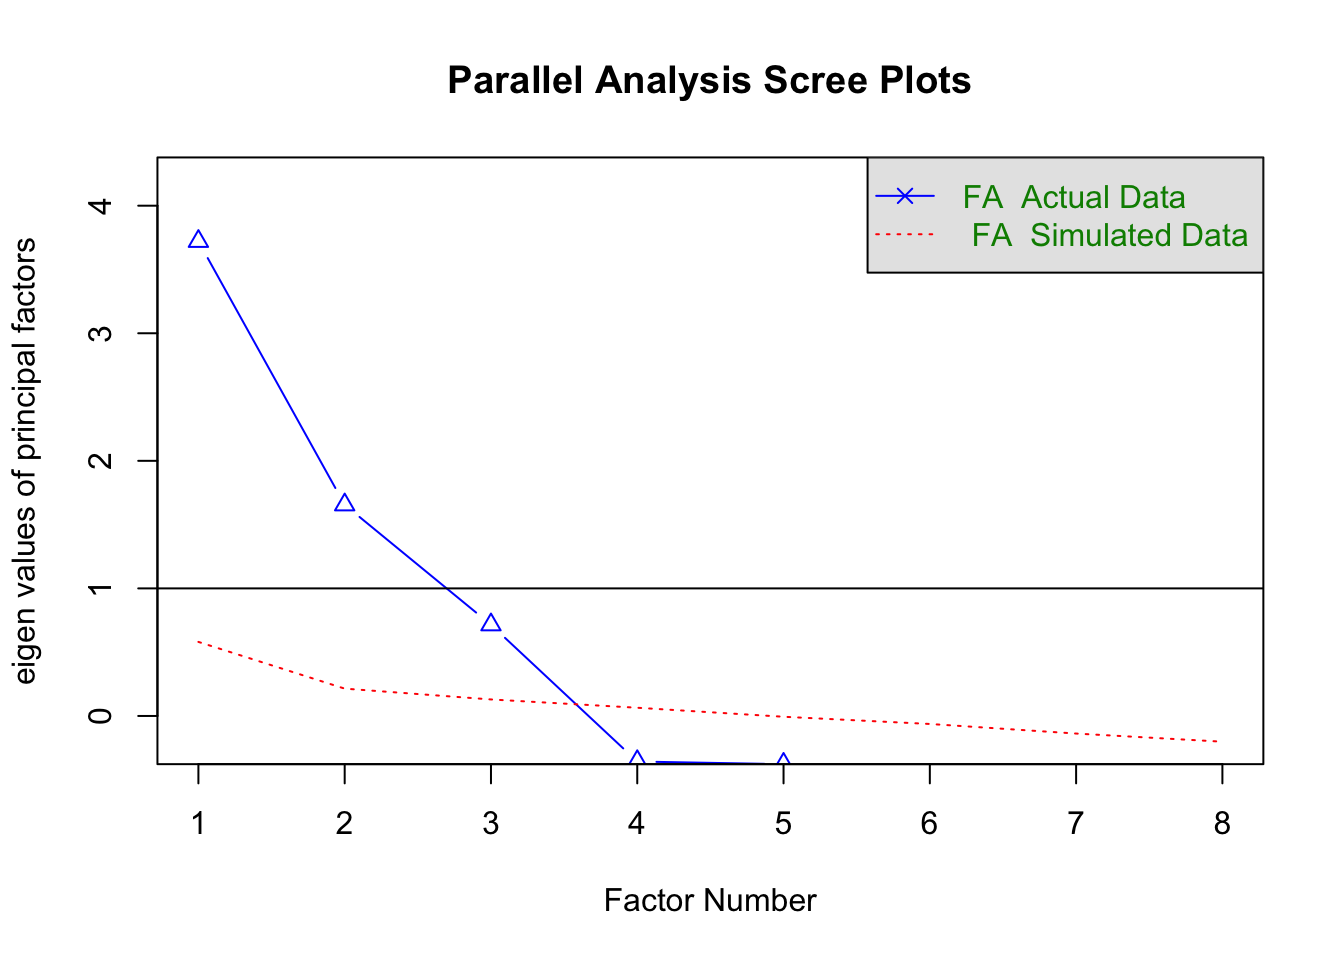
\includegraphics[width=0.4\textwidth]{../img/img34.png}}
\end{figure}
\begin{verbatim}
## Parallel analysis suggests that the number of factors =  3
## and the number of components =  NA
\end{verbatim}
De donde obtenemos que el número de factores óptimo es 3.

Terminamos AF con la siguiente visualización para saber que variables se corresponden a cada uno de los factores:
\begin{figure}[H]
\centering
\subfigure{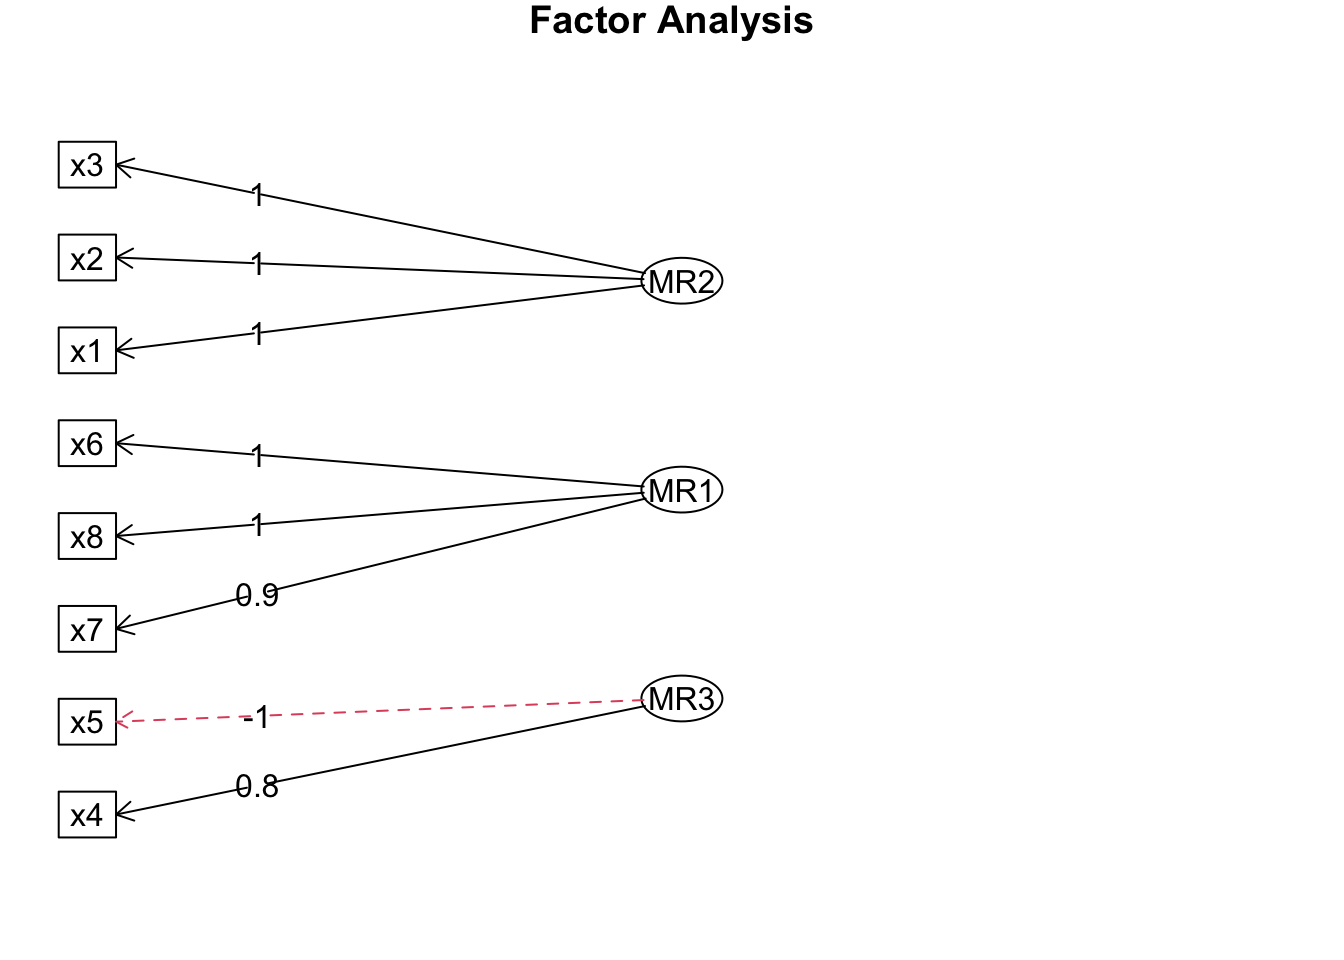
\includegraphics[width=0.6\textwidth]{../img/img35.png}}
\end{figure}

Para el análisis de normalidad multivariante, hemos utilizado los test de Royston y de Henze-Zirkler, que nos proporcionan evidencias de que siguen una distribución normal multivariante. Además, del test de Royston obtenemos la siguiente gráfica:
\begin{figure}[H]
\centering
\subfigure{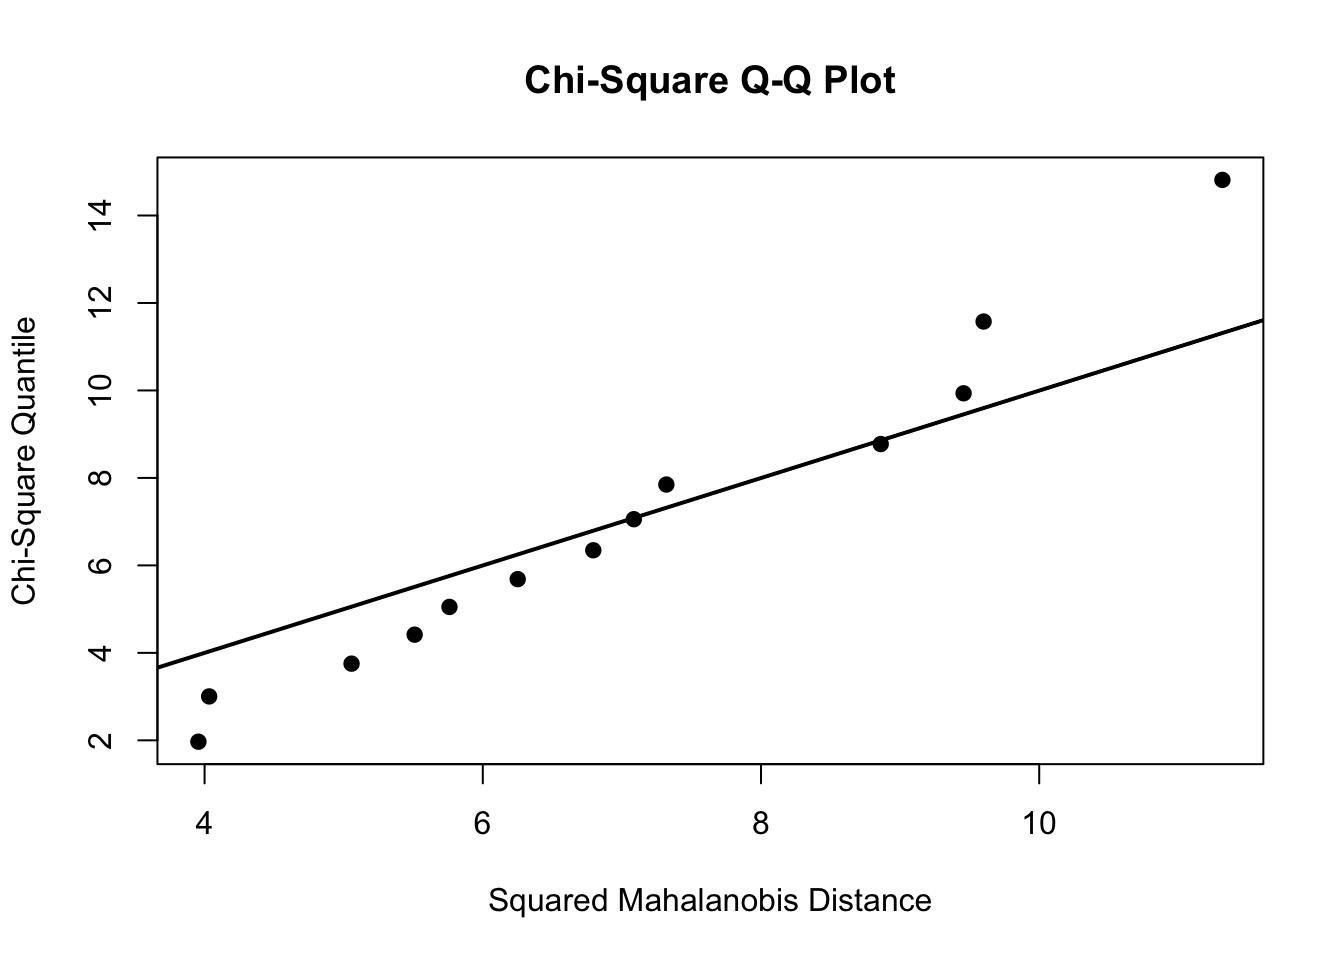
\includegraphics[width=0.5\textwidth]{../img/img37.png}}
\end{figure}

Finalmente, en el análisis clustering, comparamos los resultados obtenidos según el número de clusters utilizados:
\begin{figure}[H]
\centering
\subfigure{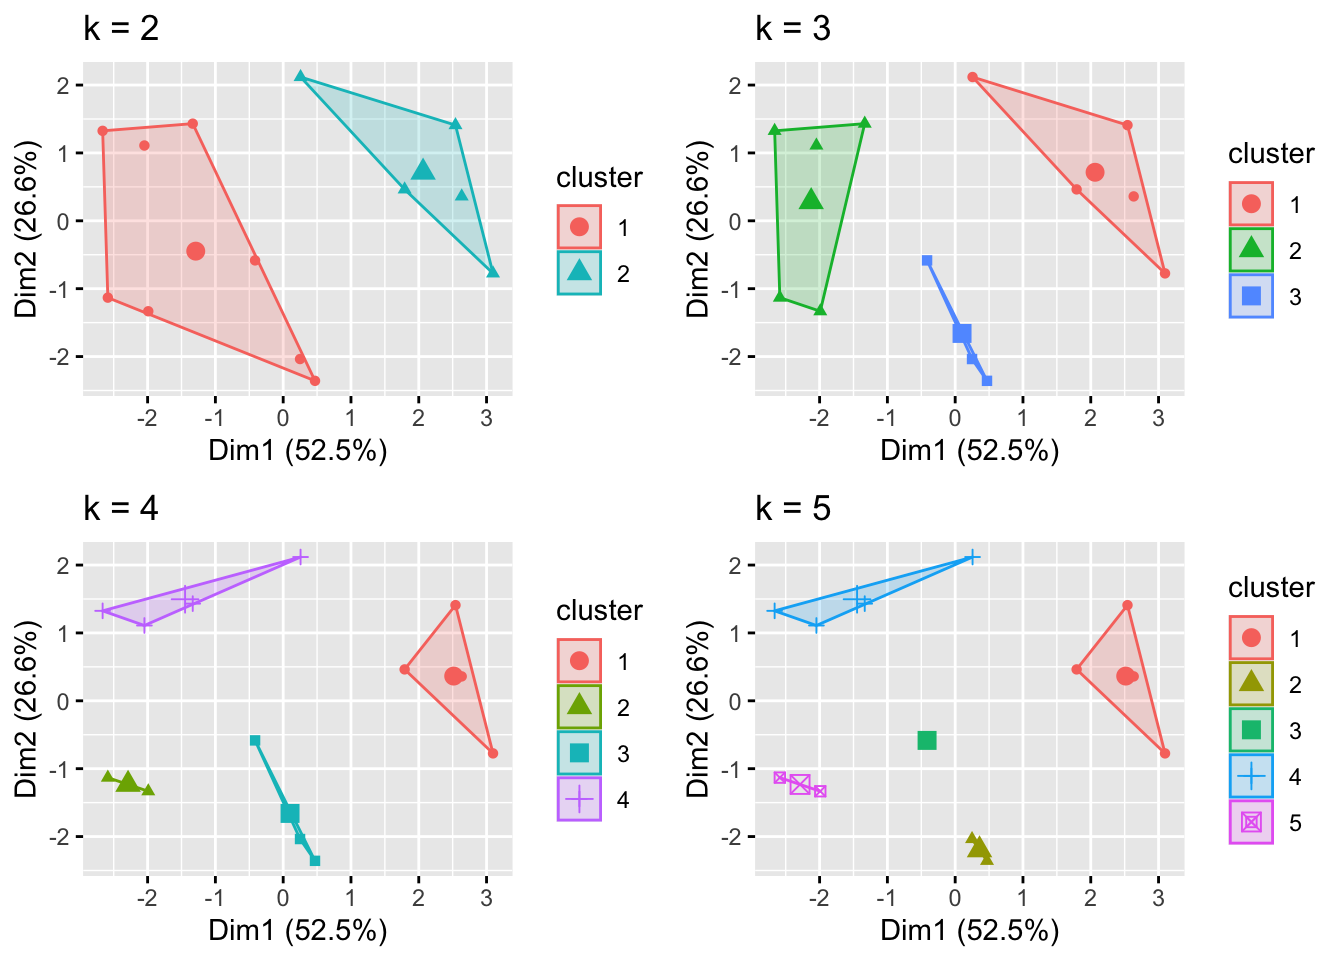
\includegraphics[width=0.65\textwidth]{../img/img39.png}}
\end{figure}

Utilizamos varios métodos para obtener el número óptimo de clusters, obteniendo las siguientes gráficas:
\begin{figure}[H]
\centering
\subfigure{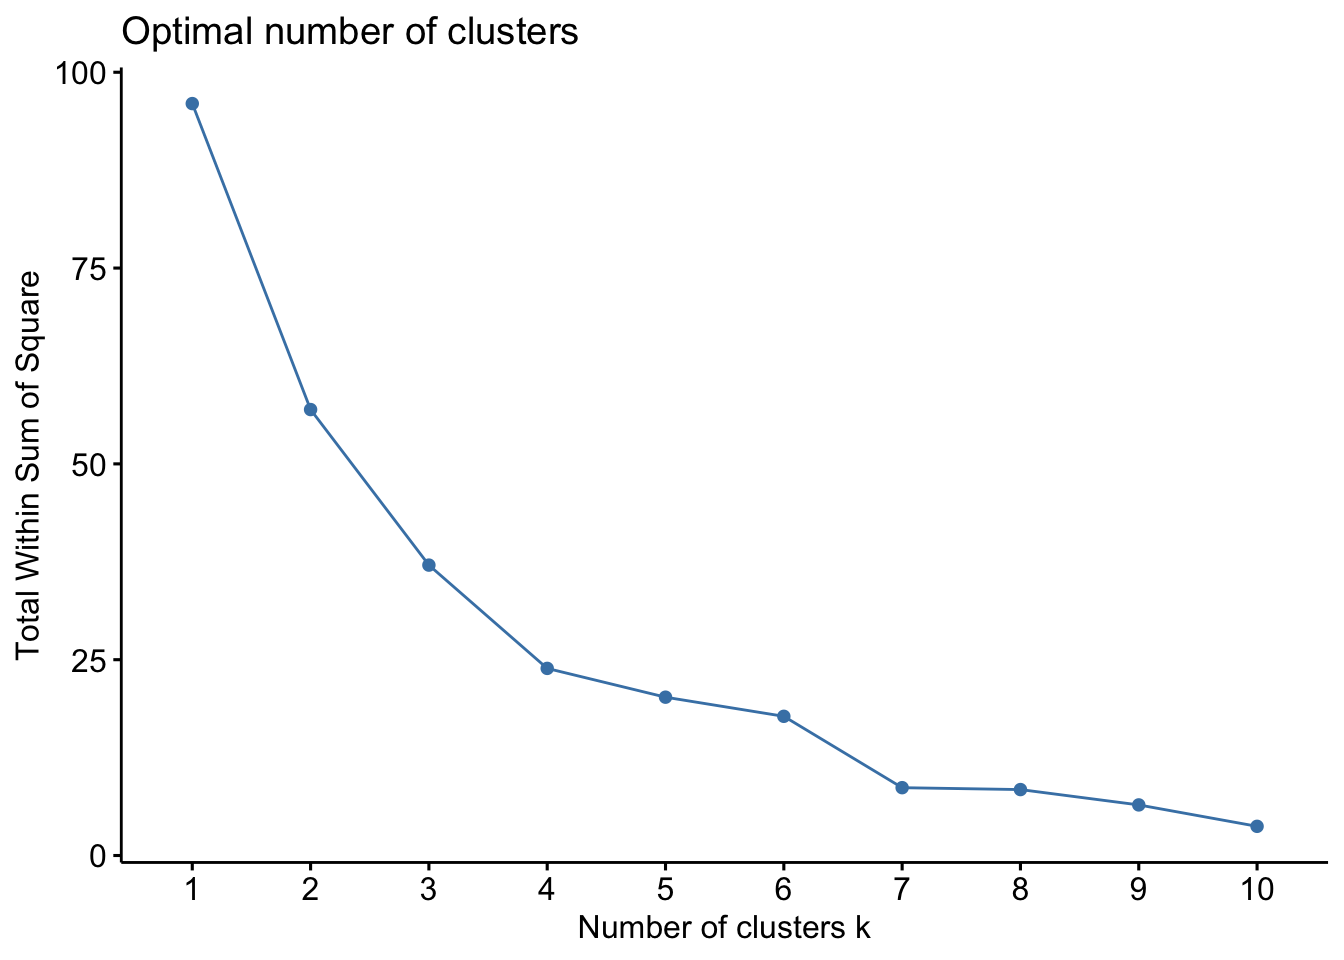
\includegraphics[width=0.3\textwidth]{../img/img40.png}}
\subfigure{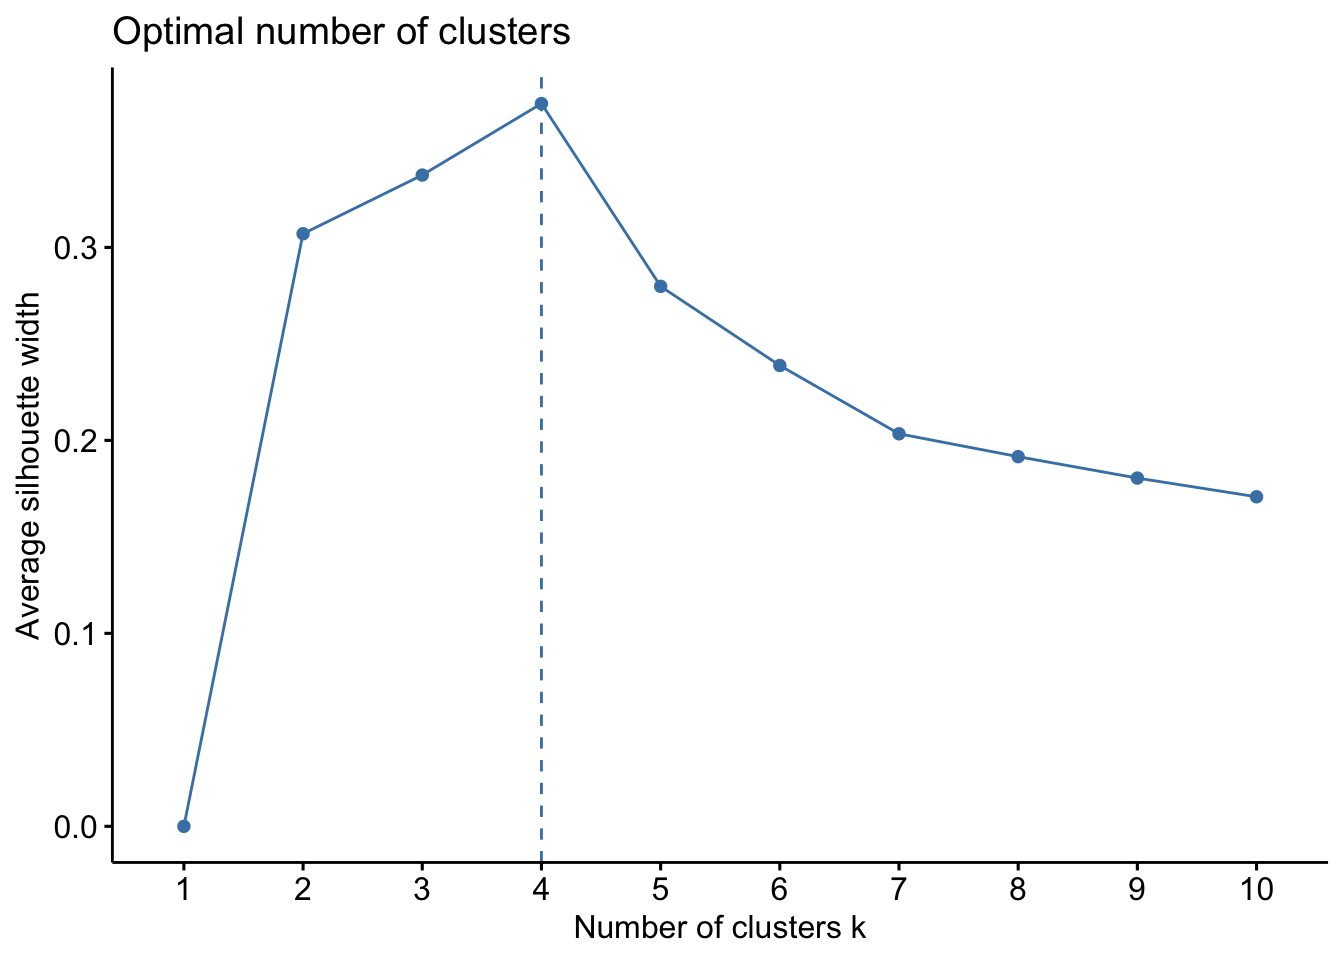
\includegraphics[width=0.3\textwidth]{../img/img41.png}}
\subfigure{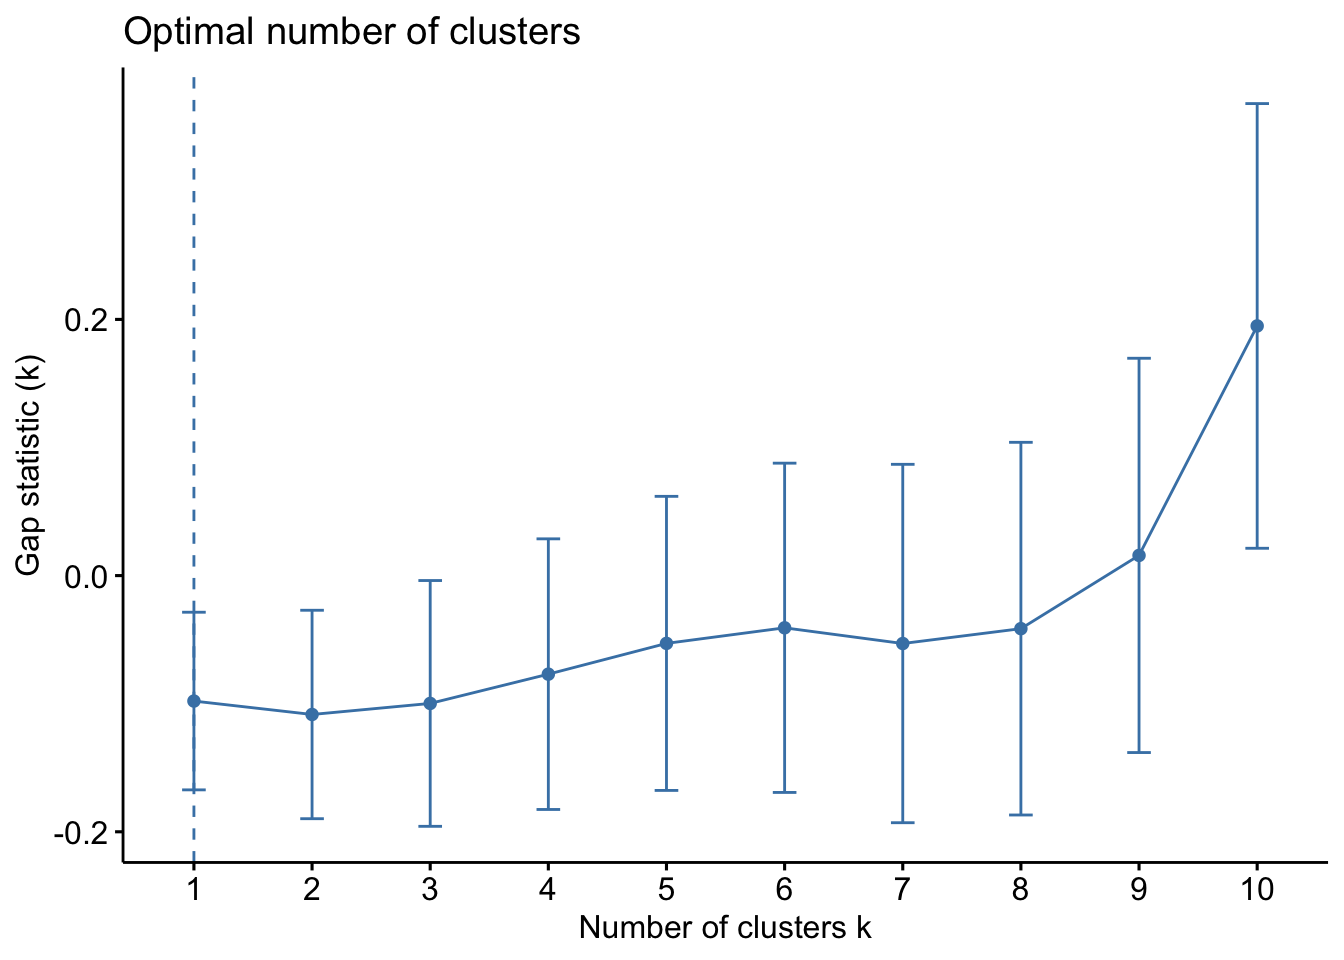
\includegraphics[width=0.3\textwidth]{../img/img42.png}}
\end{figure}

Nos decidimos por utilizar los resultados del \emph{Silhoutte}, visualizado en la gráfica previa central, de donde obtenemos 4 clusters, que nos proporciona la siguiente silueta:
\begin{figure}[H]
\centering
\subfigure{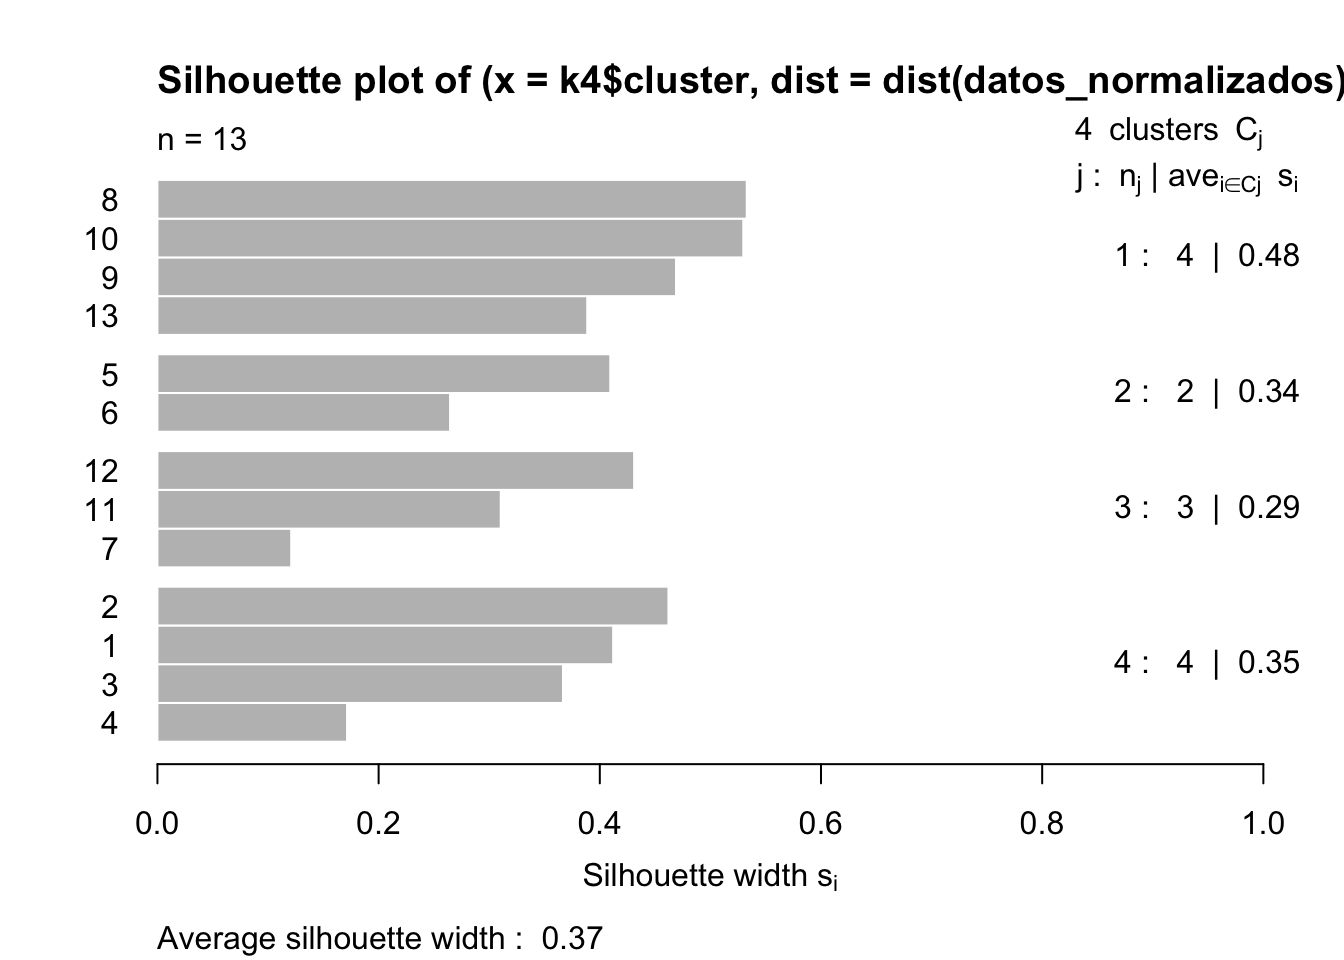
\includegraphics[width=0.6\textwidth]{../img/img43.png}}
\end{figure}

\section{Discusión y conclusión}

En primer lugar, durante el tratamiento de valores perdidos hemos encontrado una fila de más de la que nos indicaba la descripción de la base de datos que además contenía todos los valores perdidos y valores mucho mayores de los esperados, por lo que decidimos eliminarla.

Analizando el coeficiente de simetría obteníamos valores positivos y negativos. Los valores positivos indican que la distribución está sesgada a la derecha, y valores negativos indican que está sesgada a la derecha.

En el tratamiento de outliers, estudiamos los diagramas de caja, que nos indicaban que sí había algunos outliers presentes, pero con la función \emph{check\_outliers} no obteniamos ninguno, por lo que decidimos no eliminarlos, especialmente debido a los pocos datos que tenemos.

En el estudio del supuesto de normalidad obteniamos que algunas variables no se distribuyen respecto a una normal. Para detallar esto, utilizamos el test de Shaoiro-Wilk, de donde obteníamos que las variables \emph{x6} y \emph{x8} son las que nos dan problemas, ya que nos proporcionan un \emph{p-valor} inferior a 0.05:
\begin{verbatim}
## 
## $x6
## 
##  Shapiro-Wilk normality test
## 
## data:  newX[, i]
## W = 0.84811, p-value = 0.02694
## 
## 
## $x8
## 
##  Shapiro-Wilk normality test
## 
## data:  newX[, i]
## W = 0.86598, p-value = 0.04623
\end{verbatim}
El resultado con las otras variables está incluido en el archivo \emph{html}, pero debido a que sus \emph{p-valores} eran mayores del 0.05, no entramos en detalle.

En el Análisis de Componentes Principales obtenemos que el número óptimo de componentes es 3.

En el Análisis Factorial, en las gráficas obteníamos resultados contradictorios, obteniendo 2 factores en un caso y 3 en otro, pero finalmente nos decidimos por utilizar 3 factores.

El mayor problema lo obteníamos en la clasificación, con el análisis clustering, en el que cada método nos proporcionaba un número distinto de clusters. Lo más probable es que esto se debe al bajo número de instancias, ya que sólo tenemos 13, y este bajo número afecta fuertemente al clustering. Finalmente decidimos seguir los resultados de \emph{Silhouette}, ya que nos proporcionaba unos resultados claros de 4 clusters, pero sería ideal poder aumentar el número de variables antes de tomar esta decisión.

\end{document}